\documentclass[PaulGanssle-Thesis.tex]{subfiles}

\begin{document}
\chapter{Experimental Control}
\label{Chapter:Console}
\section{Overview}
\label{console.overview}
Among the significant challenges presented by the design of scientific instruments, experiment control and data acquisition can often be among the most subtle. Consoles and console software serve as the interface between scientists and the experiments they're conducting, and if poorly designed can serve as a significant barrier to usability or even limit the types of experiments that can be done where no limits might exist in the instrumental hardware. In general, well-designed systems should feel natural, and it is often the case that if users are thinking about the system at all, it's because something has gone wrong. As such these challenges are both extremely important and non-obvious.

One important factor to consider in experimental control systems is general applicability. For many systems, potential use cases will change and expand as time goes on, and so while building an ad hoc system with limited utility may be cheaper and quicker in the short run, it may cause more work in the long run. In our lab, several magnetometers were in use at the time, each using non-ideal ad hoc systems for experimental control and data acquisition, and so this console and console software was designed to be duplicated for general use on all similar systems. Additionally, because these instruments are each unique, much effort was made to make the underlying back-end as modular as possible, so that similar software could be use to control different hardware.

Our experimental control system consists of two parts - a hardware console which controls the timing of the experiment, the data acquisition and has some analog output capabilities, and software to control the console - called (imaginatively) Magnetometer Controller. Our hardware controller uses a \unit[100]{MHz} 24-channel USB PulseBlaster TTL generator for timing control (described in Sec. \ref{console.timing.pulseblaster}) and a USB-6229 BNC 16-bit, \unitfrac[250]{kS}{s} Multifunction DAQ for analog input and output (described in Sec. \ref{console.timing.nidaq}). The console software was written in ANSI C using LabWindows/CVI and is described in detail in Sec. \ref{console.software}.

\section{Timing control and analog output}
\label{console.timing}
Timing is particularly important in NMR experiments, wherein the precision with which one is able to manipulate the spins is related to the precision in the length of an excitation pulse or delay. For experiments with more than one dimension, pulse and acquisition timing becomes a critical factor in the data themselves, and in RF experiments, receiver and pulse phase are determined by how well synchronized the two timing systems are.

Likely the most important type of uncertainty present in digital timing control consoles is the digitization limit - digital devices can only change state in response to a clock pulse, and so timing is quantized into units of clock cycles. For a \unit[1]{MHz} CPU, timing cannot be controlled at a level finer than \unit[1]{$\mu$s}, whereas a \unit[100]{MHz} CPU potentially has \unit[10]{ns} resolution. For a \unit[1]{G} DC pulse, this is a difference between \unit[0.12 and 0.0012]{\degsym} pulse resolution, which can certainly add up when applying large numbers of pulses. Generally uncertainty in the absolute timing is small relative to the digitization error, and are likely to be swamped by timing errors propagating in the controlled devices. 

\subsection{Spincore Pulseblaster}
\label{console.timing.pulseblaster}
Experimental timing is all provided by a single 24-channel 200 MHz USB PulseBlaster TTL generator from SpinCore, controlled by the SpinAPI C interface. Pulse sequences consist of an array of pulse instructions, which specify the state of each TTL at each clock cycle. Each instruction consists of a 24-bit word describing the on-off state of each TTL, a 32-bit unsigned integer specifying the number of clock cycles before the next change in state, an 8-bit integer specifying the pulse instruction.

\subsection{NI-DAQ Analog Output}
\label{console.timing.nidaq}
The data acquisition system is based on a USB-6229 M-series multifunction DAQ system from National Instruments. In the current configuration of the instrument, its 4 analog outputs are used to set the DC levels of various pulse programming channels - the pulse amplifier is generally configured with one ``fixed'' DC level and one floating - with the floating channel controlled by the DAQ, though this is primarily because the USB-6229 has only 4 outputs - there would not be an appreciable increase in the noise or stability were other outputs to be used. The analog output is capable of being programmed for shaped pulses, but at the time of this writing this functionality has not yet been implemented in the software, as it was not necessary for the experiments we performed.

\section{Data Acquisition}
\label{console.daq}
% Information about the use of the DAQ.

\section{Software}
\label{console.software}
The main software used for experimental control was the Magnetometer Controller program, written in C using LabWindows/CVI. LabWindows was chosen as it has a more versatile development backend than LabView, but similar support for control of scientific instrumentation and simple interface for GUI building. In earlier versions of the program, a single event triggered the full data acquisition, preventing the use of any windowed acquisition sequences; in the latest version of the program, the acquisition of a single data point is triggered by a retriggerable internal clock waveform, allowing for arbitrary acquisition sequences.

\subsection{Pulse Programming}
\label{Section:Console-Software-PulseProgramming}
\subsubsection{Overview}
\label{Section:Console-Software-PulseProgramming-Overview}
One of the core essential functions of the console software is to serve as a simple graphical user interface for pulse programming. To define terminology, in this text, the pulse program refers to the entire set of instructions required to run an experiment - this includes both the timing and pulse controls as well as the analog output and acquisition settings. In this case this must be distinguished from the set of timing instructions executed during each acquisition\footnote{Occasionally pulse programs do not make use of a set of pulse timings - this is frequently the case when acquiring data from a continuous source like a test signal. It is presumably a semantic question as to whether a null set of instructions can be considered a set of instructions - for simplicity's sake, we shall assume that in this context it is.}. The term ``experiment'' in this context refers to the entire set of acquisitions described by the pulse program - which is not to be confused with a single acquisition (which, again, also has a plausible claim to the term ``experiment''). 

Each experiment steps through a series of acquisitions as dictated by the pulse program. At the beginning of each acquisition, the program loads a series of timing instructions into the memory of the pulse controller, initializes the values for the DAQ analog outputs and sets up an acquisition in the analog input channel of the DAQ. Generally there is much greater uncertainty associated with the timing of software triggers sent via USB than with either the DAQ or controller's internal clocks, and so it is preferable to set the DAQ waiting for a hardware trigger, which is then provided by the pulse controller - thus synchronizing the pulse timing with the acquisition. As such, the DAQ is always initialized to wait for a trigger\footnote{This is still done even when no pulse controller is used by configuring the DAQ to trigger from its own internal clock} and the DAQ acquisition task can be started immediately. The acquisition task is always started \textit{before} the pulse controller, as it ensures that the DAQ will be waiting for the trigger before it's issued by the pulse controller.

\begin{figure}[h!]

\begin{lstlisting}[style=C,escapeinside={\%*}{*},basicstyle=\scriptsize]
double ** RunAcquisition() {
	if(requires_scan) {
		SetupDAQTask();									// Configure the DAQ
		StartDAQTask();									// Start the DAQ waiting for a trigger.
	}
			
	if(pulse_controller_used) {
		pulse_controller_status = RUNNING;				
		
		StartPulseController();							
		while(pulse_controller_status != STOPPED) {		// Wait for the pulse program to finish executing.
			Wait(10 ms);								
			pulse_controller_status = GetPulseControllerStatus();	// Query the board for its status.
		}
	}
	
	if(requires_scan) {
		data[current_step] = ReadDoubleData();			// Read data as an array of doubles.
		StopDAQTask();									// Stop the task so that it can be re-created																		// in the next loop.
	}		
			
	return data;
}
\end{lstlisting}

\caption{C-style pseudocode algorithm for each acquisition.}
\label{fig:AcquisitionPseudocode2}
\end{figure}

The general algorithm seen in \ref{fig:AcquisitionPseudocode2} is executed in an asynchronous \lstinline|while| loop which checks both whether the experiment has finished its execution and whether the user has issued a stop command, prematurely terminating the operation. The parameters for each acquisition are stored in a \lstinline|cexp| (current experiment) structure, and are updated with each experiment.

\begin{lstlisting}[style=C,escapeinside={\%*}{*},basicstyle=\scriptsize,caption={The \lstinline|cexp| or \textit{current experiment} structure, which contains the parameters of a given experiment.},label={fig:CEXPStructPseudocode}]
typedef struct CEXP {
	TaskHandle aTask; 		// Signal acquisition task
	TaskHandle cTask;		// Counter task.

	int update_thread;		// Update thread id.
	
	PPROGRAM *p;			// Current program
	
	int nchan;				// Number of channels.
	int t_first;			// Transients first or indirect aq first?
							// Three options: 	0 -> ID first, then advance transients.
							//					1 -> All transients first, then ID
							//					2 -> Phase Cycles first, then IDs, then repeat as necessary
	
	char *path;				// Full pathname of where to save the data
	char *fname;			// Experiment filename.
	char *bfname;			// Base filename
	unsigned int num;		// Experiment number. 
	char *desc;				// Description of the experiment.
	
	dstor data;				// Cached data
	dstor adata;			// Cached data average
	
	char *ctname;			// Counter task name
	char *atname;			// Acquisition task name
	
	char *ccname; 			// Counter channel name
	char **icnames; 		// Input channel names
	
	int ctset;				// Whether or not the counter task has been set
	int atset;				// Whether or not the acquisition task has been set.

	int cind;				// Current index
	unsigned int steps_size;// Number of values in *steps
	unsigned int *cstep;	// Same size as steps
	unsigned int *steps;	// Maxsteps -> It will have one of three forms:
							// 1: !p->varied -> steps = [nt]
							// 2: MC_TMODE_ID [{dim1, ..., dimn}, nt]
							// 3: MC_TMODE_TF [nt, {dim1, ... dimn}, nt]
							// 4: MC_TMODE_PC [{pc1, ... , pcn}, {dim1, ..., dimn}, nt/npc]

							
	int ninst;				// Number of instructions in this run
	PINSTR *ilist;			// List of instructions for this run.

	time_t tstart;			// Time started
	time_t tdone; 			// Time that the most recent part was completed.
	
	double t_el;			// Elapsed time
	double t_prog;			// Amount of time taken by just the pulse program
	double t_rem;			// Remaining time on the pulse program
	double t_tot;			// Total time the program should take
	
	// Analog output info
	TaskHandle oTask;		// Analog output task

	char *otname;			// Analog output task name
	
	int otset;				// Whether or not analog output task is set
	int nochans;			// Number of analog output channels.
	int *ochanson;			// Analog output channels on. Size = nochans, Refers to indices in p->ao_chans
	char **ocnames;			// Analog output channel names. Size = nochans.
	float64 *ao_vals;		// Analog output values for each channel. Size = nochans;
	
	int64 hash;				// Current experiment hash - generated from the experiment name.
} CEXP;
\end{lstlisting}

Experiments can be multi-dimensional, include multiple transients and use multiple phase cycles, and so there are multiple approaches to the order of sampling (i.e. the conversion between our linearly-stepped index and the position in the multi-dimensional sampling space). Different experiments will call for a different order - for example, if drift over the course of an experiment is important, it may be preferable to acquire all points along a given dimension first, then repeat the entire sequence multiple times rather than acquiring all transients before moving on to the next step in the indirect dimension; on the other hand, if the noise characteristics tend to change but the signal is fairly constant, it may be preferable to sample the full phase cycle immediately, so that the noise will optimally cancel out. Although it makes things slightly more complicated, it was sufficiently important to address these different cases that the software is written such that three sampling options are available: indirect dimensions first [default], transients first, phase cycles first. In the first option, all points along indirect dimensions are acquired first before moving on to the next transient; in the second option, all transients are acquired before moving on to the next step in the sampling space; in the third option, the minimum number of transients required to execute a full phase cycle are performed, then the experiment is moved to the next step in the sampling space and that entire block is repeated to satisfy the specified number of transients.

\subsubsection{Simple Pulse Programs}
\label{console.software.simple.pulse.programs}
The core element of the experiment is a set of pulse instructions. The simplest pulse programs consist of a single set of instructions executed with or without an acquisition. These instructions are specified using a graphical interface to the Spincore PulseBlaster. Each instruction consists of 24 flags specifying the on/off state of each TTL (only 23 are user-accessible and 1 is reserved for acquisition triggering), the duration of the instruction (maximum value 21 seconds), the instruction type and a data parameter used for some instructions.

\begin{figure}[!h]
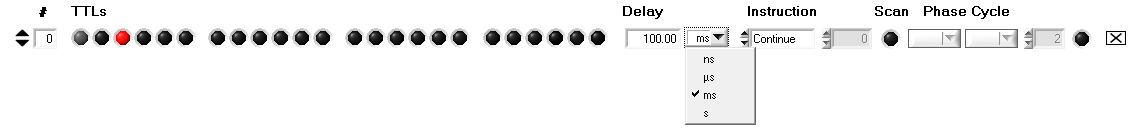
\includegraphics[width=\textwidth]{figures/console/PulseInstruction.png}
\caption{A single pulse instruction.}
\label{fig:SinglePulseInstruction}
\end{figure}

There are 8 instruction types which can be programmed into the board, which are detailed in \Cref{table:PulseBlasterInstructions} - each instruction can be no shorter than \unit[100]{ns} and no longer than \unit[21]{s}\footnote{Specifically, the instructions can be no longer than \unit[$10\cdot{}2^{31}$]{ns}. Though it is not specified in the promotional materials, this is likely because the clock cycles are counted using a signed 32-bit integer, which has a range of $\pm{}2^{31} \approx 2.1\cdot{}10^{9}$; as clock cycles are \unit[10]{ns} long, this gives a limit of $\approx$ \unit[21]{s}.}, with \unit[10]{ns} resolution. For delays longer than \unit[21]{s}, the  \textit{Long Delay} instruction type can be used, which repeats a single instruction $n$ times, where $n$ is specified using the instruction data parameter. While there was some early work done on establishing a mechanism for specifying custom instructions, which would be useful for updating things like pulse length calibrations and the like, no such system has been implemented at the time of this writing.

\def\insdtw{0.65\tw}
\begin{table}[h!]
\centering
\begin{tabular}[0.90\textwidth]{|E{0.125\tw}|E{0.125\tw}|D{\insdtw}|}
\hline Instruction & Data & \multicolumn{1}{m{\insdtw}|}{Description} \\ \hline
\textit{Continue} & Unused & \multicolumn{1}{m{\insdtw}|}{Set TTLs then wait specified duration.} \\ \hline
\textit{Stop} & Unused & \multicolumn{1}{m{\insdtw}|}{Stop the pulse program - does not update TTLs before instruction, and TTLs remain at previoiusly-specified values} \\ \hline
\textit{Loop} & Number of iterations & \multicolumn{1}{m{\insdtw}|}{Start a loop - execute this instruction and all instructions up to and including the instruction specified \textit{End Loop} whose instruction data parameter matches} \\ \hline
\textit{End Loop} & Loop instruction & \multicolumn{1}{m{\insdtw}|}{The final instruction to include in a loop started by the \textit{Loop} instruction at the position specified by the instruction data parameter.} \\ \hline
\textit{JSR} & Instruction & \multicolumn{1}{m{\insdtw}|}{Jump to a subroutine which starts at the instruction specified int he data parameter.} \\ \hline
\textit{RTS} & JSR Instruction & \multicolumn{1}{m{\insdtw}|}{Return from a subroutine to the execution of the program.} \\ \hline
\textit{Branch} & Instruction & \multicolumn{1}{m{\insdtw}|}{Sets TTLs to specified levels, waits duration, then jump to the instruction specified by the instruction data parameter. This is generally used to loop indefinitely.} \\ \hline
\textit{Long Delay} & Number of repetitions & \multicolumn{1}{m{\insdtw}|}{This is equivalent to a \textit{Continue} instruction, except that it is repeated a number of times specified in the instruction data parameter. It is used for single-instruction delays longer than 21 seconds, as single instructions cannot be longer than 21 seconds.} \\ \hline
\textit{Wait} & Unused & \multicolumn{1}{m{\insdtw}|}{Sets TTLs to specified levels, waits the duration specified, and then wait for a hardware or software trigger. This cannot be used as the first instruction, and must occur at least \unit[100]{ns} after the program begins.} \\ \hline
\end{tabular}
\caption{Spincore Pulseblaster instruction types.}
\label{table:PulseBlasterInstructions}
\end{table}

\begin{figure}[!h]
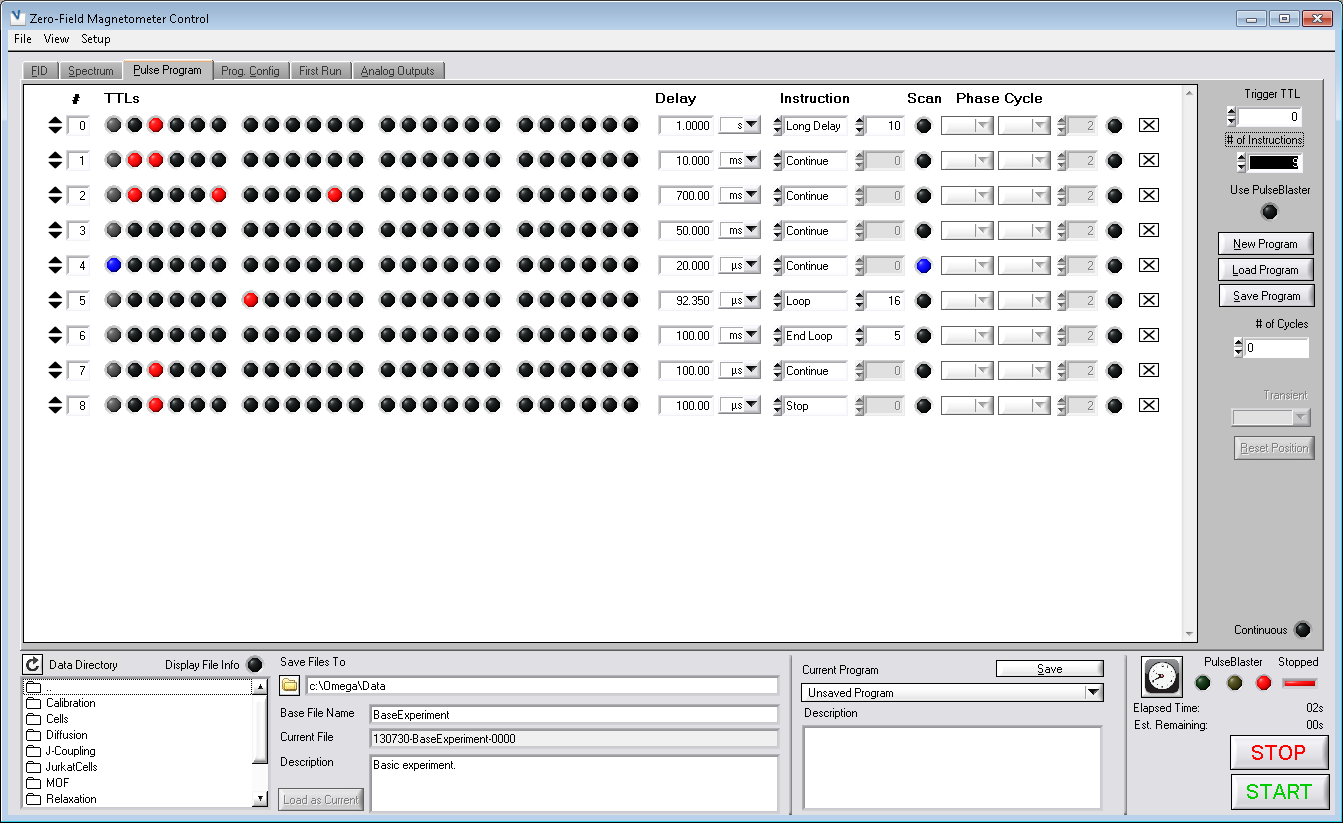
\includegraphics[width=\textwidth]{figures/console/pulse_program_1d.png}
\caption{The \textit{Pulse Program} tab for a basic experiment.}
\label{fig:PulseProgramTab1d}
\end{figure}

The basic set of pulse instructions is specified on the \textit{Pulse Program} tab. A basic example program is shown in \Cref{fig:PulseProgramTab1d} - this is a pulse program in 8 steps. The first step is a \unit[10]{s} pre-polarization time, implemented as a \textit{Long Delay} which repeats \unit[1]{s} units 10 times. I have generally found it preferable to use durations under \unit[5]{s} when possible. The second instruction turns on the leaving solenoid (TTL 1\footnote{TTLs are numbered using a zero-based index.}) while leaving the sample in the magnet for an additional \unit[10]{ms} (vacuum is controlled with TTL 2). The next instruction is the shuttling time - during this instruction a back-pressure of air is turned on along with the pulse coil along the \textbf{z} direction(TTL 10) - these are left on for a transit time of \unit[700]{ms}. The fourth instruction is a \unit[50]{ms} delay allowing the magnetometer spins to re-polarize before any measurements are taken, this is followed by a scan trigger (TTL 0), which is configured at \unit[20]{$\mu$s}. The sixth and seventh instructions are the measurement loop - 16 \unit[180]{$^\circ$} pulses are applied at \unit[100]{ms} intervals. The penultimate instruction is used to shuttle the sample back into the pre-polarizing magnet, and the final instruction stops the pulse sequence; because \textit{Stop} instructions do not change the TTL state before stopping the program, the configuration specified in the previous instruction will persist after the instructions have been executed.

\begin{figure}[!h]
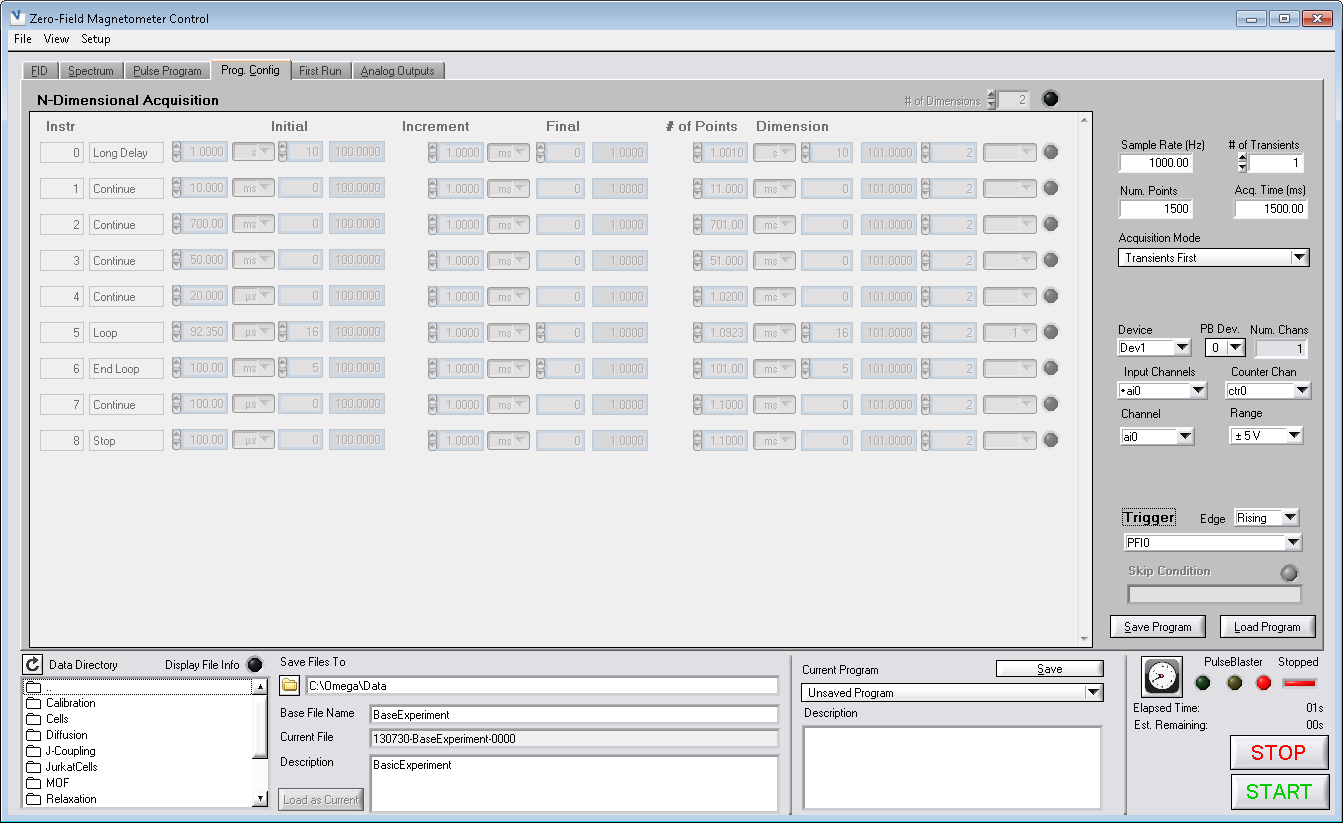
\includegraphics[width=\textwidth]{figures/console/program_config_1d.png}
\caption{The \textit{Prog. Config} tab for a simple 1D program.}
\label{fig:ProgConfigTab1d}
\end{figure}

Beyond the triggering, the acquisition parameters are configured in the \textit{Prog. Config} tab - shown in \Cref{fig:ProgConfigTab1d} for our example pulse program. The sampling rate is set to \unit[1]{kHz} as that is the value of the low-pass filter on the preamp so that no aliasing occurs. The acquisition time, number of points and sample rate are related by the equation $NP = AT/SR$, and so setting any two uniquely determines the third, in the interface, right-clicking on one of these three boxes pulls up a context menu allowing the user to specify which of the other two quantities to hold constant when updating the selected box; since the sampling rate is generally related to the signal bandwidth and analog filtration, it's usually best to configure number of points and acquisition time to hold the sampling rate constant. The number of transients box determines the number of times each step in the acquisition (in any number of dimensions) will be repeated. This value is constrained by the phase cycling, which is discussed in \Cref{console.software.phase.cycling}.

The other boxes in the acquisition configuration refer to the parameters of the actual devices, and are specific to Spincore and National Instruments devices\footnote{the program may work for other devices as generic functions are used, but they have only been tested with Spincore's 24-TTL USB Pulseblaster and the National Instruments USB-6229M devices}. The \textit{Device} and \textit{PB Dev.} pulldowns are used for selecting between multiple devices plugged into the same computer and generally will only have one option. Up to 8 input channels\footnote{This is a software limit imposed to limit the number of LED controls on the data display, and could easily be expanded if necessary. I have never used more than 2 channels at once.} can be selected via the \textit{Input Channels} pulldown - channels that are turned on will be marked with a dot, and selecting these will toggle them off. Each channel can be configured to a different sensitivity; USB-6229M DAQs support only 4 possible ranges: \unit[$\pm$0.1]{V}, \unit[$\pm$1]{V}, \unit[$\pm$5]{V} and \unit[$\pm$10]{V}. The \textit{Channel} control selects which channel's sensitivity is being configured.

As described in \Cref{Section:Console-Software-PulseProgramming}, the acquisitions are initialized before the pulse programmer is activated and waits for any number of hardware triggers. There are a number of potential channels for triggering, but may of these are virtual devices. When triggering using a PulseBlaster, it is best to use one of the 4 digital input channels (PFI0-PFI3); when using an internal trigger, the 20MHzTimeBase or 80MHzTimeBase virtual channels tend to work well. To allow the task to be retriggerable, a virtual counter channel is used to trigger individual the acquisitions of actual points; the NI USB-6229M DAQ supports 2 of these virtual channels, which are named ctr0 and ctr1, and which one of these is used can be selected using the \textit{Counter Chan} control.

To avoid the possibility that data would be lost, data are automatically saved to a new file after each acquisition. The location of these files can be specified easily using the embedded text boxes at the bottom of the magnetometer controller window. The filenames are built automatically using the current date and the specified base experiment name, currently this is set with a hard-coded definition in the library \lstinline|DataLibPriv.h|, and is set to \lstinline|MCD_FNAME_FORMAT = %s-%s-%04d| with the first string specified by the date format \lstinline|MCD_FNAME_DATE_FORMAT = %y%m%d|, the second string is the base filename and the integer is the first number which would not overwrite an existing file; this could easily be moved into a preferences dialog and changed to a user-controlled setting.

\subsubsection{Phase Cycling}
\label{console.software.phase.cycling}
Phase cycling is a technique which in general is used to control the phase coherences producing signal in an experiment. The most common application of phase cycling is to correct for artifacts in the system which are independent of the relationship between the phase of the transmitter and receiver - the quintessential phase cycling sequence is the CYCLOPS\cite{Keeler2013} method (shown in Fig. \ref{fig:CyclopsPhaseCycle}), where the phase of the transmitter phase over a multiple of 4 transients follows the sequence \textit{x}, \textit{-x}, \textit{y}, \textit{-y}, while the receiver follows \unit[90]{$^\circ$} behind. When the transients are averaged, signals whose phase relative to the receiver add, while all others average out, leaving things like NMR precession (whose phase is always \unit[90]{$^\circ$} away from the transmitter phase) and eliminating signals such as detector asymmetries and signal offsets.

\begin{figure}[!h]
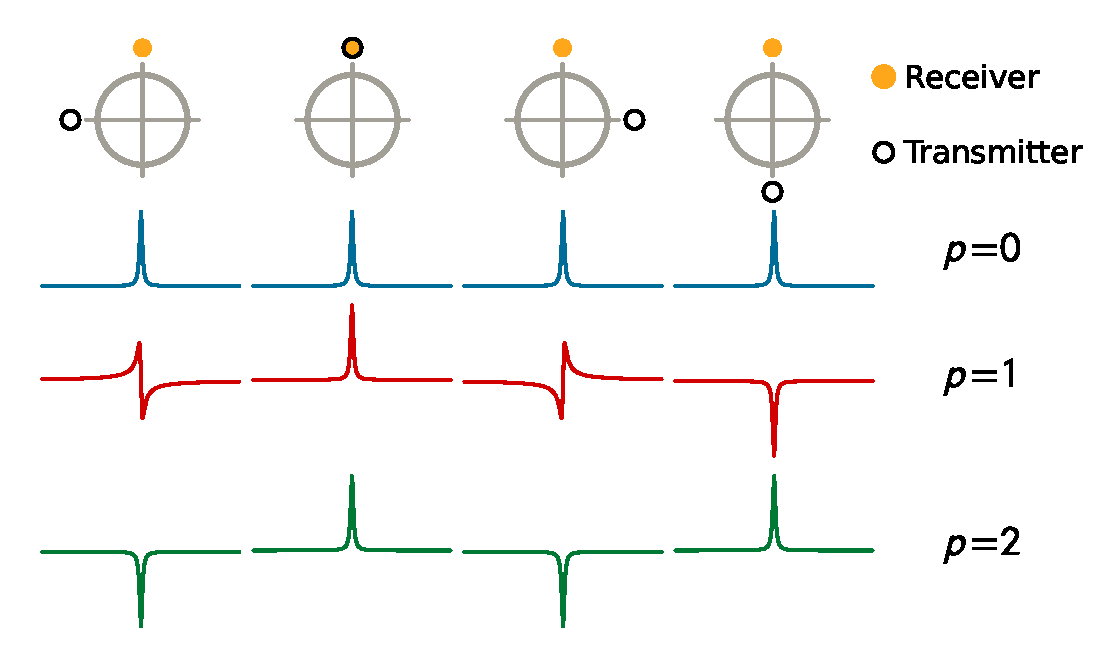
\includegraphics[width=\textwidth]{figures/console/CYCLOPS.eps}
\caption{A demonstration of the CYCLOPS phase cycling sequence. Over the course of four transient acquisitions, the transmitter phase is varied while the receiver phase is held constant. In this scheme, coherences of order $p \neq 0 \mod{4}$ average out, while coherences with order $p = 0 \mod{4}$ are unaffected.}
\label{fig:CyclopsPhaseCycle}
\end{figure}

This same concept still has significant applicability at zero field, where phase corresponds to a direction in the lab frame, but phase encoding can be somewhat more complicated in a regime with a carrier frequency of zero and two distinct methods of phase cycling need to be implemented. One use for phase cycling for low-frequency acquisitions is to remove discrete noise, such as the ever-present \unit[60]{Hz} noise and its many harmonics. When the acquisition is started at a random time with respect to a source of discrete noise, the noise averages out over multiple transients due to changes in the phase of the acquired waveform, which averages away slightly slower than $\sfrac{1}{\sqrt{N}}$ for a random distribution of phases. If the experiment is instead triggered using a source synced to the problematic discrete noise, the phase of the noise can be deliberately chosen such that it will average out over the course of the acquisitions. Choosing $n$ phases evenly sampled from the interval $[0, 2\pi)$, the signal contribution from the $m^{th}$ harmonic is given by:

\begin{equation}
\sum_{k}^{n}\cos{(\sfrac{2\pi\cdot{}k\cdot{}m}{n})}
\end{equation} 

Which sums to 0 for all harmonics $m \not\equiv 0 \bmod{n}$. In the console software, this is generally accomplished by using a \lstinline|Wait| instruction followed by a \lstinline|Continue| instruction with a duration which is varied to sample all multiples of $\sfrac{1}{nt\cdot{}f}$ where $f$ is the frequency of the noise source and $nt$ is the number of transients acquired in the cycle; the hardware is then triggered on a function generator synced to the noise source. In general, it is preferable to sample in phase-alternated pairs so that drift or other changes over time do not interfere with the phase averaging (e.g. for a four-phase cycle it is preferable to sample 0,$\pi$, $\sfrac{\pi}{2}$, $\sfrac{3\pi}{2}$ as the maximum cancellation happens between pairs separated by a phase of exactly $\pi$). This helps to minimize the effect of a trigger source which is imperfectly synchronized with the noise source; as the time between experiments is often several orders of magnitude longer than the period of the noise source, even small deviations from the ideal frequency can grow quickly and reduce the effectiveness of this technique. By choosing phase cycles in pairs, the phase drift between experiments is limited to the length of one experiment.

The other primary use of phase cycling in the context of zero-field NMR would be to eliminate potential artifacts due to pulse direction. This may be useful in a number of contexts where the absolute phase of the experiment is chosen arbitrarily, such as the quadrature and vector detection schemes described in Sections \ref{nmr.signal.magnetization.quadrature} and \ref{nmr.signal.magnetization.vector} respectively. In the vector detection scheme, for example, measurements can be made $x-x-y-y$ or $y-y-x-x$, with some signal decay in whichever is detected second; by phase cycling between the two possibilities, the decay artifact can be reduced or eliminated.

The interface to specify phase cycling in the console is built into the basic pulse program instruction GUI and is shown in Figure \ref{fig:PhaseCycleInstructionCollapsedLabeled}. A \textit{phase cycle} here refers to a full repetition of all the chosen phases; most experiments with phase cycling will have exactly one phase cycles, but it is possible to compound phase cycles together as is necessary for some coherence pathway selection sequences, or to eliminate discrete noise \textit{while} adjusting for directional artifacts. Phase cycling can be enabled using the LED control to the far right of each instruction, doing so enables a pulldown control and automatically increments the number of cycles to 1 if it is set to zero.

\begin{figure}
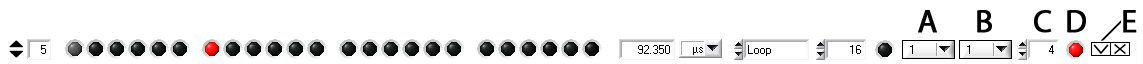
\includegraphics[width=\tw]{figures/console/PhaseCycledInstructionCollapsed01Labeled.png}
\caption{The initial state of a phase cycled instruction when phase cycling is turned on. The instruction to display is selected using the pulldown labeled \textbf{A}. \textbf{B} is used to select the phase cycle along which this instruction should vary. \textbf{C} sets the number of steps in the phase cycle (and updates all other instructions varying along the same cycle). \textbf{D} toggles phase cycling on and off, and \textbf{E} is used to collapse or expand the full phase cycle view.}
\label{fig:PhaseCycleInstructionCollapsedLabeled}
\end{figure}

Phase cycling on an instruction is enabled using an LED control (labeled \textbf{D} in Fig. \ref{fig:PhaseCycleInstructionCollapsedLabeled}), which allows a different instruction to be set for each step in the phase cycle. This can be done either by selecting and modifying the instructions one at a time by cycling through the pulldown labeled \textbf{A}, or by expanding the instruction to see all steps by using the expander control labeled \textbf{E} - bringing up the interface shown in Fig. \ref{fig:PhaseCycleInstructionExpanded}. The number of steps in a cycle can be set using the control labeled \textbf{C}, which changes the number of steps for all instructions with the same cycle. To add additional cycles, the ``number of cycles'' control on the \textit{Pulse Program} tab must be incremented. The phase cycle along which a given instruction is varied is set by the control labeled \textit{B}.

\begin{figure}[!h]
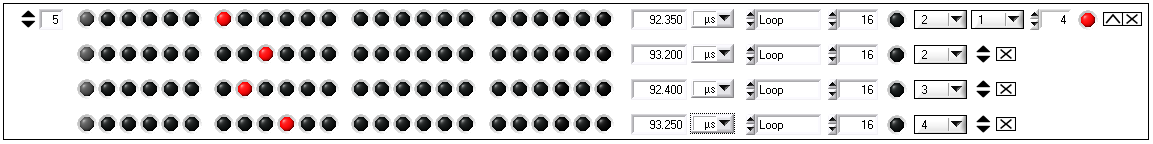
\includegraphics[width=\tw]{figures/console/PhaseCycledInstruction.png}
\caption{The expanded view for a 4-step phase cycle, which cycles a $\pi$ pulse between $x$, $y$, $-x$ and $-y$.}
\label{fig:PhaseCycleInstructionExpanded}
\end{figure}

Because of the difficulty of implementation and the low need for such a thing, it is currently not possible to vary a single instruction both along an indirect dimension and as part of a phase cycle. In most cases it is possible to replicate this functionality using two separate instructions, however. Because the actual type of instruction can be varied as part of a phase cycle, it is possible to use a \lstinline|JSR| instruction to specify a different subroutine for each cycle, and the instructions in that subroutine can be varied along an indirect dimension if need be. This functionality has not been tested, however, and so it is not clear what its versatility is. Because it is not possible to simultaneously view the \textit{Pulse Program} and \textit{Prog. Config.} tabs, instruction numbers for phase cycled instructions are highlighted in red on the \textit{Prog. Config.} tab as a reminder.

As phase cycling is intended to be averaged out, the phase cycle step is encoded in the transient step; as such, the number of transients in an experiment must be an even multiple of $\prod_{i}^{nc}ns_{i}$ where $nc$ is the number of phase cycles and $ns_{i}$ is the number of steps in cycle $i$. When the number of phase cycle steps is changed the number of transients is automatically changed to be the closest multiple to the previous value of the transient and the control is changed such that the up and down arrow keys increment the number of transients by the minimum number of transient steps.

\subsubsection{Multidimensional Acquisition}
\label{console.software.ndacq}
\begin{figure}[!h]
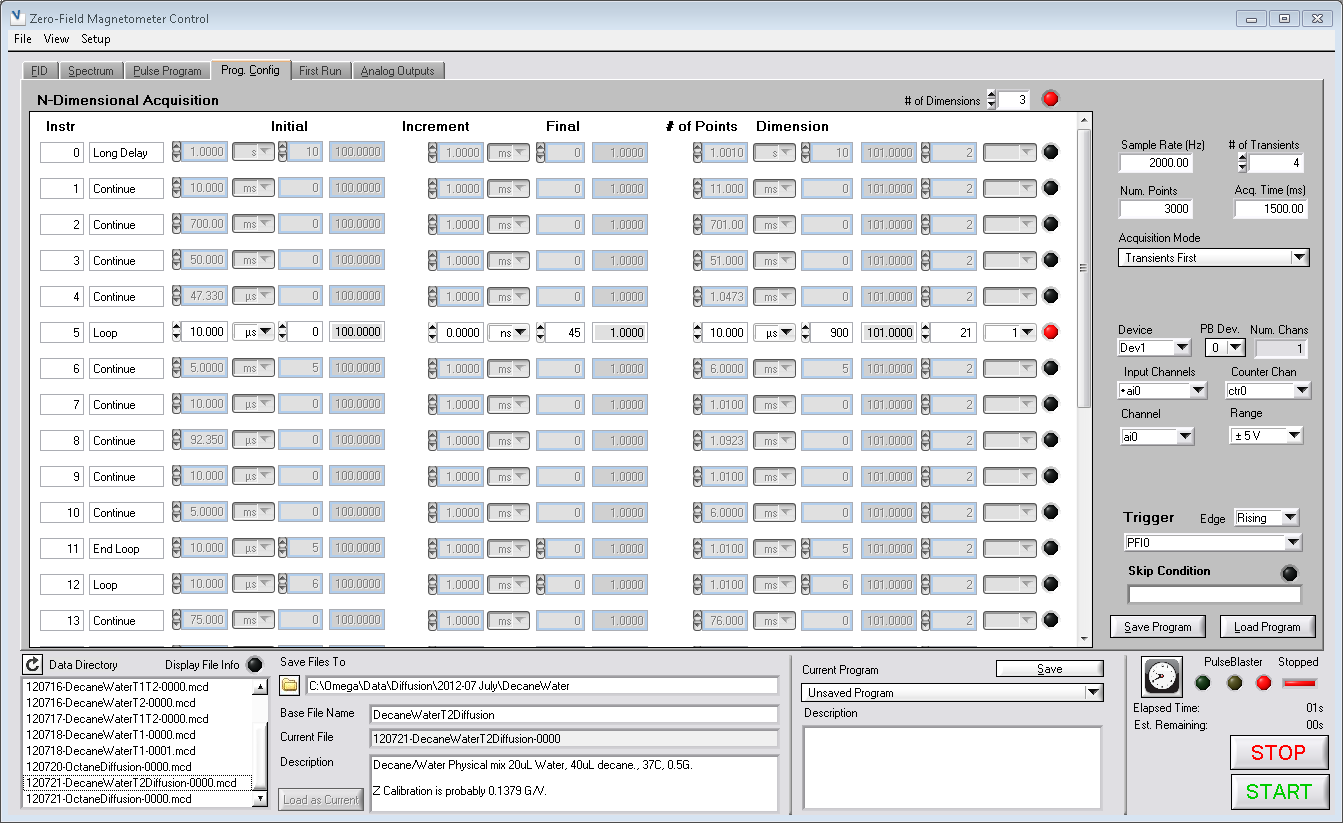
\includegraphics[width=\tw]{figures/console/program_config_2d.png}
\caption{The \textit{Prog. Config.} tab for a 3-dimensional experiment for running a T$_{2}$-diffusion experiment in an indirect dimension. The mis-positioning of the labels is due to a cosmetic bug that had not been fixed at the time of this writing.}
\label{fig:ProgConfigTab2D}
\end{figure}
Many experiments we've been interested in performing are multi-dimensional experiments, such as the relaxometry and diffusometry experiments described in Chapter \ref{relaxometry}, which are performed in a second, indirect dimension. These acquisitions are again specified using a graphical user interface which allows for a number of types of variation. Multi-dimensional acquisitions are mostly configured on the \textit{Prog. Config.} tab, and can be enabled with the \textit{\# of Dimensions} control and associated LED. When the LED is enabled, the ND control panel is enabled, and the ND-state of the instructions can be toggled (see Figure \ref{fig:ProgConfigTab2D}). In this control, the direct dimension is considered one of the dimensions.

The \textit{N-Dimensional Acquisition} panel contains a list of the instructions each with an associated LED control (\textbf{K} in Fig. \ref{fig:PulseInstruction2D}) for toggling the variation mode. There are three possible modes: no variation [0], linear variation [1] and equation-based variation [2]. Left-clicking toggles in a positive cycle (0$\rightarrow{}$1$\rightarrow{}$2$\rightarrow{}$0), and right clicking toggles in the opposite direction (0$\rightarrow{}$2$\rightarrow{}$1$\rightarrow{}$0). These LEDs are color-coded, with a red control indicating linear variation and blue indicating equation-based variation.

\begin{figure}[!h]
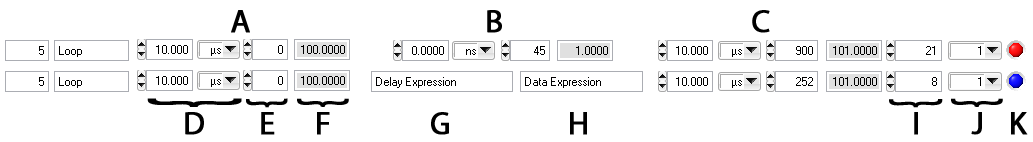
\includegraphics[width=\tw]{figures/console/PulseInstruction2D.png}
\caption{A pulse instruction for linear variation (top) and equation-based variation (bottom). Labels are described in the text.}
\label{fig:PulseInstruction2D}
\end{figure}

Each instruction can be varied either in the delay, data or both. An example of both a linear and equation-based instruction is shown in Figure \ref{fig:PulseInstruction2D}. In some cases, multiple instructions need to vary along the same direction, so the dimension of variation can be specified using a pulldown control (\textbf{J}); the number of steps in the selected dimension can be updated from control \textbf{I} on any instruction varying along the specified dimension.

Each instruction is divided into three components, the initial value (\textbf{A}), the increment value(\textbf{B}) and the final value (\textbf{C}). Since there are three controls and only 2 degrees of freedom, when one is changed, at least one of the other two is recalculated. In the case of linear variation, the update is hard-code such that changing the initial value or increment updates the final value, and changing the final value updates the increment. This is hard-coded into the callbacks \texttt{ChangeInitOrFinal} and \texttt{ChangeInc} in the primary function library \texttt{MC10.c} and can be easily changed in the code. In equation-based variation, both the initial and final values are calculated from the equation, and so both are updated - these values can also be used in the equations, and so caution must be taken to ensure that any variables used are not changed upon evaluation\footnote{One such example would be the equation \texttt{init+3}, which sets all values - including the initial value - to be 3 units greater than the initial value. This will result in the initial value being incremented by 3 upon each evaluation}. While in the \textit{Pulse Program} instructions an instruction can be no shorter than \unit[100]{ns}, this restriction is lifted in the multi-dimensional case to allow for instructions to be omitted entirely - any instruction length shorter than \unit[100]{ns} will be skipped, as will \texttt{Loop} and \texttt{Long Delay} instructions of length 0. The upper limit of \unit[21]{s} is still enforced. Increments can also take on negative values as they represent a change in time rather than an absolute time.

Each value specification in Figure \ref{fig:PulseInstruction2D} is broken into three components, the duration (\textbf{D}), data parameter (\textbf{E}) and instruction length (\textbf{F}). The duration can be specified in any units from nanoseconds to seconds and changing the unit specifier will change the value in the numeric control such that the total duration does not change - which is in contrast to the unit specifier on the \textit{Pulse Program} tab, which in fact keeps the numeric control constant and changes the real duration; while it is often not ideal GUI design to have identical-seeming controls with different behavior, these choices were made based on the most common use case in each context. The \textbf{F} control is not user-specified, but rather is an experimental control which attempts to calculate the total duration of a given instruction. This was implemented to make more obvious the duration of a loop instruction whose data parameter is varying.

\begin{figure}[!h]

\includegraphics[width=\tw]{figures/console/expression_mode_data_expr.png}
\caption{A pulse instruction where the data parameter is varied according to an equation. In this case, stepping through powers of two.}
\label{fig:EquationAcceptedDataMode}
\end{figure}

For equation-based variation, I wrote a math parsing library which reads in a small number of variables. When the equation has been entered into controls \textbf{G} and/or \textbf{H}, it is evaluated for all the real values in the experiment\footnote{This can take some time, as the math parser has not been optimized, and relies heavily on redundant and costly string-processing operations. I have written a new algorithm for much faster math parsing, but it has yet to be implemented.} and checked for errors. Functions which have been accepted with no errors will display a green background (as seen in Fig. \ref{fig:EquationAcceptedDataMode}), while functions with errors will display a red background. The variables available for use in the equations are detailed in Table \ref{table:EquationVariables}, and should be displayed as a tooltip by stalling the mouse over an expression control.

\def\eqvardw{0.8\tw}
\begin{table}[h!]
\centering
\begin{tabular}[0.90\textwidth]{|E{0.1\tw}|D{\eqvardw}|}
\hline Variable & \multicolumn{1}{m{\eqvardw}|}{Description} \\ \hline
\lstinline|nd| & \multicolumn{1}{m{\eqvardw}|}{The total number of dimensions (including the direct dimension)} \\ \hline
\lstinline|nc| & \multicolumn{1}{m{\eqvardw}|}{The number of phase cycles} \\ \hline
\lstinline|x| / \lstinline|step| & \multicolumn{1}{m{\eqvardw}|}{Two aliases for the current step in the dimension [unused in skip equations]} \\ \hline
%\lstinline|cds[n]| & \multicolumn{1}{m{\eqvardw}|}{Current step for dimension \lstinline|n|. In this case, a zero-based index is used, and so \lstinline|n| takes values from 0 to \lstinline|nd-2|\footnote{As the direct dimension counts as a dimension, it is included n \lstinline|nd|, but beause it does not vary in steps, it is not included in this variable.}. The exact format is always \lstinline|cds%d|, so these will be \lstinline|cds0|,\lstinline|cds1|, etc.} \\ \hline
\lstinline|ccs[n]| & \multicolumn{1}{m{\eqvardw}|}{Current step for phase cycle \lstinline|n|. Again, a zero-based index is used, so \lstinline|n| spans from 0 to \lstinline|nc-1|.} \\ \hline
\lstinline|mds[n]| & \multicolumn{1}{m{\eqvardw}|}{Maximum number of steps in dimension \lstinline|n|.} \\ \hline
\lstinline|mcs[n]| & \multicolumn{1}{m{\eqvardw}|}{Maximum number of steps in phase cycle \lstinline|n|.} \\ \hline
\lstinline|init| & \multicolumn{1}{m{\eqvardw}|}{The initial value specified in the instruction [not used in skip equations]. Since this control is updated from the equation, care must be taken to ensure that at step 0, this evaluates to exactly \lstinline|init|.} \\ \hline
\lstinline|final| & \multicolumn{1}{m{\eqvardw}|}{The final value specified in the instruction [not used in skip equations]. As with \lstinline|init|, care must be taken to ensure that the equation evaluates to \lstinline|final| at the last step.} \\ \hline
\lstinline|us| & \multicolumn{1}{m{\eqvardw}|}{Durations are specified in nanoseconds, so this is an alias for 10$^{3}$, to specify $\mu{}s$.} \\ \hline
\lstinline|ms| & \multicolumn{1}{m{\eqvardw}|}{Alias for $10^{6}$, for specifying milliseconds.} \\ \hline
\lstinline|s| & \multicolumn{1}{m{\eqvardw}|}{Alias for $10^{9}$, for specifying seconds.} \\ \hline
\end{tabular}
\caption{Variables available for math parsing applications during pulse programming.}
\label{table:EquationVariables}
\end{table}

Most arithmetic and boolean operations are supported, with the order of operations detailed in Table \ref{table:EquationOperators}. Trigonometric functions such as $\sin()$ and $\cos()$ are not implemented, nor are complex functions. Equations always return doubles which are rounded down by conversion to \lstinline|int| when used in the data parameter; boolean true returns 1.0 and boolean false returns 0.0, while all non-zero values evaluate to boolean true. Using boolean operations and comparators, it is possible to create rudimentary conditional statements; for example, to implement a delay which increases by \unit[300]{ms} each step until it reaches \unit[1.5]{s} with the algorithm described in this pseudocode:

\begin{lstlisting}
if(cds0*300*ms <= 1.5*s) {
	return cds0*300*ms;
} else {
	return 1.5*s;
}
\end{lstlisting},

the equation would be set as:

\begin{lstlisting}
(cds0*300*ms <= 1.5*s)*(cds0*300*ms) + (cds0*300*ms > 1.5*s)*(1.5*s)
\end{lstlisting}.

Since these are mutually exclusive and span all cases, this is equivalent to the above pseudocode, as either the comparison on the left evaluates to 1.0 and the comparison on the right evaluates to 0.0 or the opposite is true.

\def\eqopdw{0.65\tw}
\begin{table}[h!]
\centering
\begin{tabular}[0.95\textwidth]{|E{0.2\tw}|E{0.1\tw}|D{\eqopdw}|}
\hline Operation & Order & \multicolumn{1}{m{\eqopdw}|}{Description} \\ \hline
\lstinline|()| & 1 & \multicolumn{1}{m{\eqopdw}|}{Parentheses for equation grouping.} \\ \hline
 \lstinline|exp()|, \lstinline|log()| & 2 & \multicolumn{1}{m{\eqopdw}|}{Exponential and natural logarithm functions} \\ \hline
 \lstinline|^| & 3 & \multicolumn{1}{m{\eqopdw}|}{Exponentiation} \\ \hline 
\lstinline|*|,\lstinline|/|, \lstinline|%| & 4 & \multicolumn{1}{m{\eqopdw}|}{Multiplication, division and modulo} \\ \hline
\lstinline|+|,\lstinline|-| & 5 & \multicolumn{1}{m{\eqopdw}|}{Addition and subtraction} \\ \hline
\lstinline|&|,\lstinline!|! & 6 & \multicolumn{1}{m{\eqopdw}|}{Bitwise AND and OR} \\ \hline
\lstinline|=|,\lstinline|!=| & 7 & \multicolumn{1}{m{\eqopdw}|}{Comparators $=$ and $\neq$} \\ \hline
\lstinline|>=|, \lstinline|>|, \lstinline|<=|, \lstinline|<| & 7 & \multicolumn{1}{m{\eqopdw}|}{Comparators $\geq$, $>$, $\leq$ and $<$} \\ \hline
\lstinline|!|, \lstinline|&&|, \lstinline!||!, \lstinline|<| & 8 & \multicolumn{1}{m{\eqopdw}|}{Boolean operators: Negation, AND and OR.} \\ \hline
\end{tabular}
\caption{The order of operations and supported syntax. Operations are executed according to the \textit{Order} column, generally top-to-bottom.}
\label{table:EquationOperators}
\end{table}

\subsubsection{Subsampling}
\label{Section:Console-Subsampling}
One problem with the multi-dimensional acquisition setup is that it is designed to only acquire along a grid (whether linear or non-linear), when often it would be preferable to sample only a subset of such a grid. For example, in T$_1$/T$_2$ acquisitions, values are generally sampled along each of the two dimensions from \unit[0]{s} to $3\cdot$T$_1$ or $3\cdot$T$_2$ and signal varies according to $e^{-t_{1}/T_{1}}e^{-t_{2}/T_{2}}$ where $t_{1}$ is the time step in the T$_{1}$ dimension and $t_{2}$ is the time step in the T$_{2}$ dimension. At the point where $\sfrac{t_{1}T_{2}+t_{2}T_{1}}{T_{1}T_{2}} \geq 3T_{1}T_{2}$, there is nearly no signal - which in the case of the standard sampling pattern is fully half of the points in the sampling space. What's worse, it is the \textit{longer} half; for T$_{1}$ = T$_{2}$ = \unit{1.5}[s], sampling 25 points in each direction from 0 to \unit[4.5]{s} with a \unit[10]{s} re-polarization time and a \unit[2]{s} measurement time takes \unit[2]{h}\unit[51]{m}\unit[53]{s}, but when all values such that $t_{1}T_{1}+t_{2}T_{2} \geq 3\cdot{}T_{1}T_{2}$ are skipped, the same experiment can be acquired in only \unit[1]{h}\unit[21]{m}\unit[15]{s}, saving an hour and a half while discarding only transients which are contributing very little to the signal.

This functionality is implemented in the GUI in the form of \textit{Skip Expressions}, which is an optional box on the \textit{Prog. Config.} tab in which an expression can be entered. The same parser described in Section \ref{console.software.ndacq} is used to process these equations, and the syntax and relevant variables can be found in Tables \ref{table:EquationOperators} and \ref{table:EquationVariables} respectively.  The equation is evaluated as a boolean value for each point in the acquisition with all non-zero values evaluating to boolean true; if the skip expression evaluates to true for a given point in the acquisition space, this point is skipped. These boolean values are stored in an array and saved with the data to allow the reconstruction of the original acquisition grid during data processing.

\subsubsection{Analog Output Controls}
\label{console.software.analog.output}
\begin{figure}[!h]
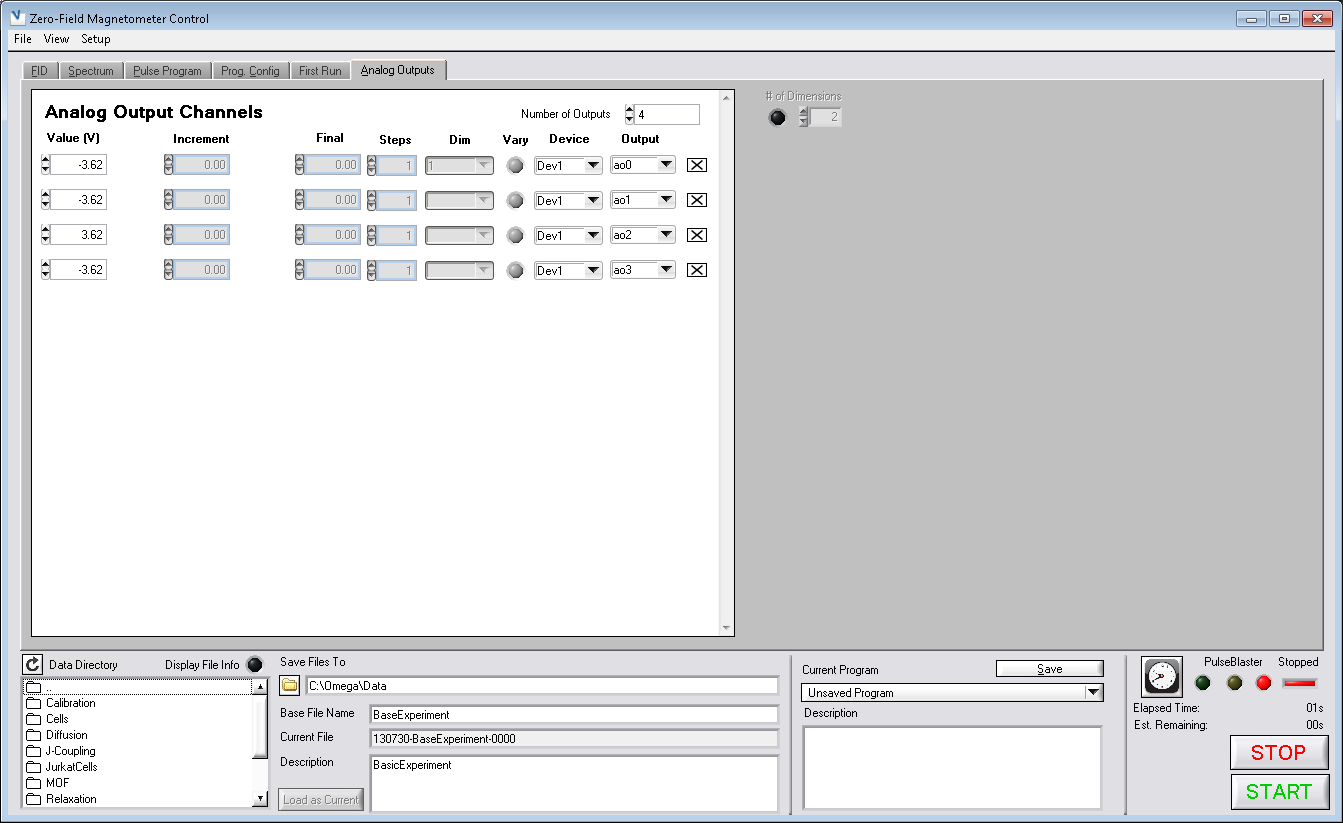
\includegraphics[width=\tw]{figures/console/AnalogOutput1d.png}
\caption{The \textit{Analog Output} tab, used to set analog output levels and variation.}
\label{fig:AnalogOutputTab1D}
\end{figure}
The National Instruments USB-6229M DAQ has 4 analog outputs, which are currently used in our console to control the DC pulse levels for the pulser output channels. It is also possible to use these to apply shaped pulses or low-frequency waveforms, but this functionality is not currently supported in the console control program. The analog output channels on any number of devices can be set using the \textit{Analog Output} tab, shown in Figure \ref{fig:AnalogOutputTab1D}. Each analog output can take values from \unit{-10}[V] to \unit[10]{V}. To add an analog output, increment the \textit{Number of Outputs} control and then select the Device and Output Channel from the respective pulldowns. Selecting an output from a given device removes it from the other pulldowns so that there will be no conflicts when attempting to set the output levels.

\begin{figure}
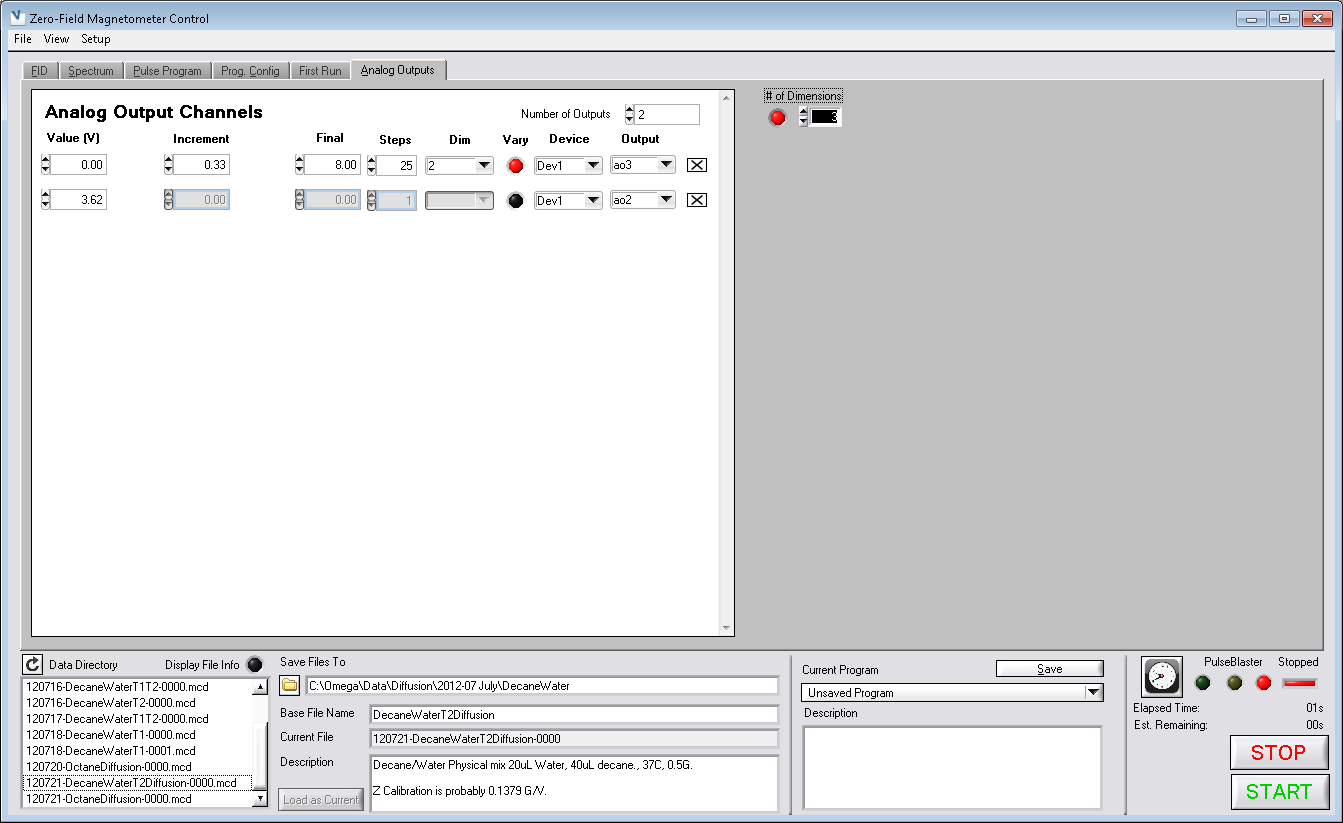
\includegraphics[width=\tw]{figures/console/AnalogOutput2d.png}
\caption{A multi-dimensional experiment which varies an analog output channel as a function of one of the indirect dimensions.}
\label{fig:AnalogOutputTab2D}
\end{figure}

These analog outputs can also be varied along an indirect dimension which might be used to set gradient strengths or sweep a bias offset field, for example. When multi-dimensional acquisitions have been activated using the LED and numeric control on either the \textit{Prog Config.} or \textit{Analog Outputs} tabs, the \textit{Vary} LED control will be activated on each analog output channel. At the moment, only linear variation of analog outputs is supported. The dimensions and dimension number specified in the \textit{Prog. Config} tab are equivalent to those specified in the \textit{Analog Output} tab, and as such it is possible to vary both an instruction and an analog output along the same or different indirect dimensions; this means that changing the number of steps for a shared dimension on either tab will update the number of steps and increments on the other, and so care should be taken that this does not cause any issues when switching between tabs.

\subsubsection{First and Last Runs}
\label{console.software.first.runs}
\begin{figure}[!h]
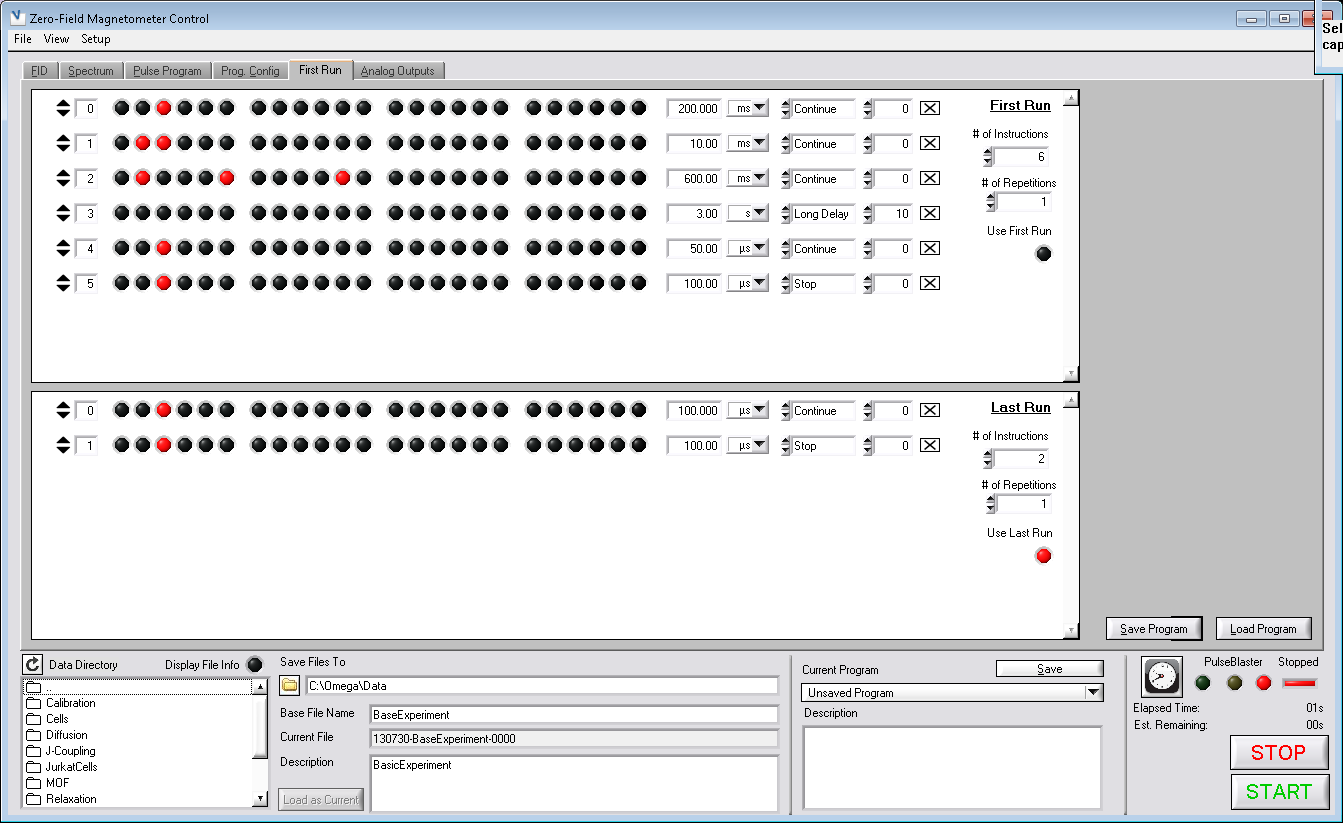
\includegraphics[width=\tw]{figures/console/FirstRun.PNG}
\caption{The \textit{First Run} tab, used to set the first and last runs in an acquisition}
\label{fig:FirstRunTab}
\end{figure}

Occasionally during the course of an experiment, the sample or system will undergo an equilibration process, usually due to differences in temperature between the prepolarization region and the detection region. This can cause problems with the first few data points before the system reaches a steady state. To avoid these equilibration problems, it is sometimes best to run a few ``dummy'' experiments without taking any data. This functionality is implemented in the \textit{First Run} tab, shown in Figure \ref{fig:FirstRunTab}, which contains a first and last run instruction set.

The top panel is used to build the instruction set for the dummy runs, which can be repeated an arbitrary number of times using the \textit{\# of Repetitions} control. The instruction set will be saved regardless of whether or not it is used, and so its use can be toggled using the \textit{Use First Run} LED control.

This tab also contains a last run panel - this was implemented primarily because of a bug in the PulseBlaster which tends to trigger whatever experiment is loaded into memory occasionally when the chassis voltage changes suddenly (which tended to happen due to static buildup on a person's fingers when the optical table was touched). To prevent a long sequence with many pulses from activating on its own, the Last Run was generally set to a simple pulse program which kept the shuttle from sampling. This was loaded into memory and run 1 time after the pulse sequence. It is not possible to acquire data during either the first or last run.

\subsection{Data Display}
\label{console.software.display}
\begin{figure}[!h]
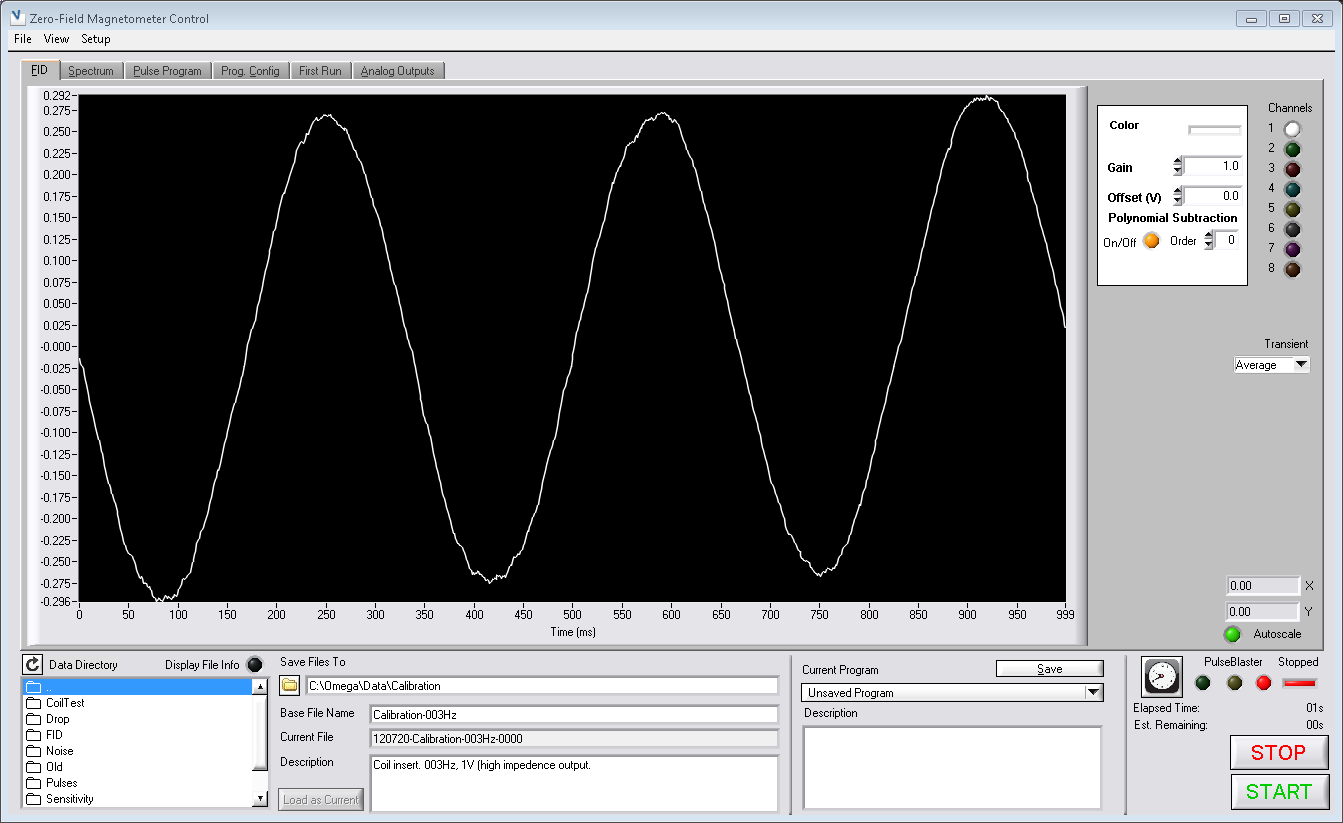
\includegraphics[width=\textwidth]{figures/console/FIDDisplay1D.png}
\caption{The \textit{FID} tab, which displays data in the time domain.}
\label{fig:FIDDisplay1D}
\end{figure}

While most data is likely to be analyzed in MATLAB or an equivalent platform, it can also be read and manipulated to some extent directly in the console program. Data is displayed automatically upon acquisition using the most recent settings, or can be loaded from the File>Load menu or using the navigation box in the bottom left hand corner of the program.

The data can be displayed only in one dimension, either in the time (FID) domain (Figure \ref{fig:FIDDisplay1D}) or in the frequency domain (Figure \ref{fig:FFTDisplay1D}). Up to 8 channels can be independently displayed, each with its own user-configurable line color, gain, offset and polynomial subtraction settings. Setting the order of the polynomial subtraction to 0 subtracts off the data mean. In the FID domain, polynomial subtraction is applied, followed by gain, then offsets. In the frequency domain, polynomial subtraction is applied to the time domain data before Fourier transformation, then gain, then offsets. When polynomial subtraction is turned on in a given channel, it is turned on in both the time domain and the frequency domain, while gain and offsets are set independently. Data are assumed to be in units of volts.

\begin{figure}[!h]
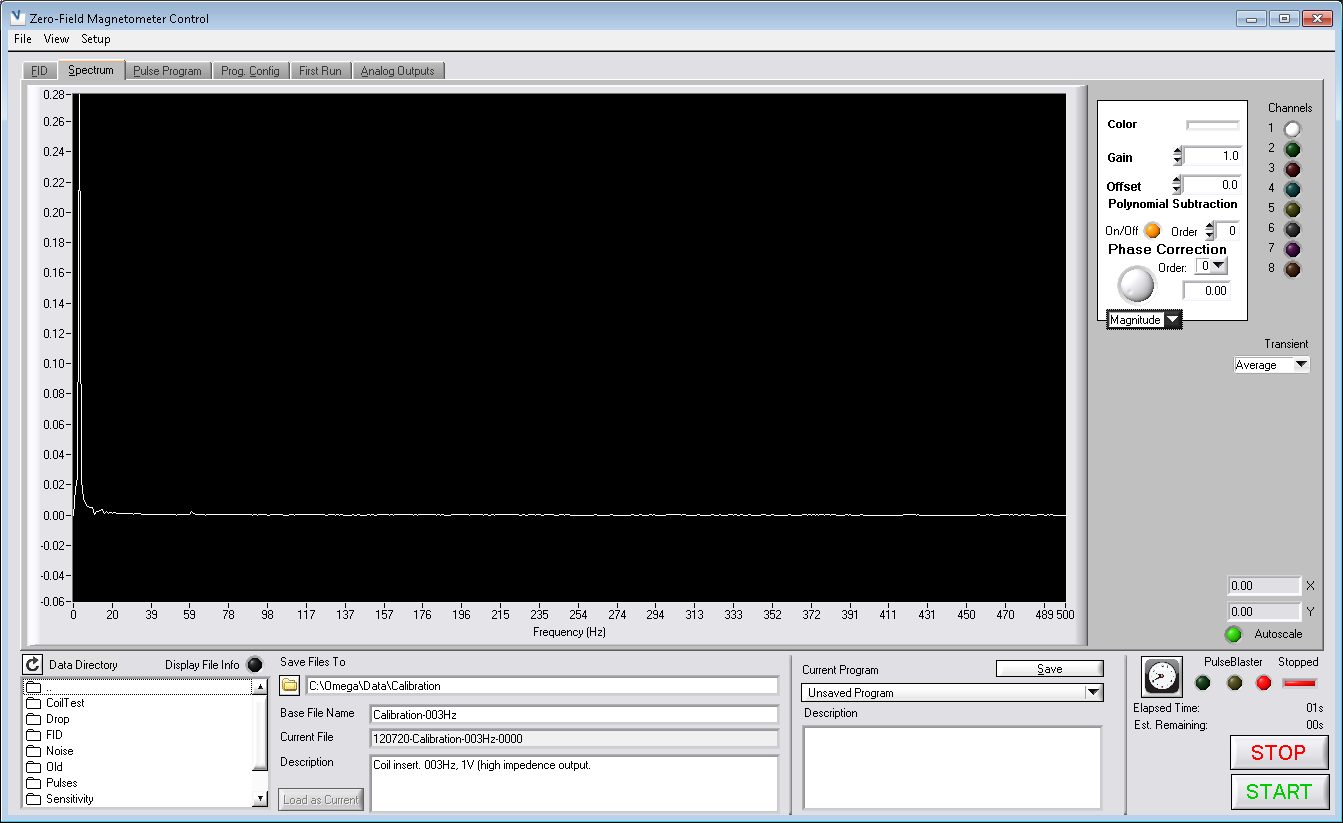
\includegraphics[width=\textwidth]{figures/console/FFTDisplay1D.png}
\caption{The \textit{FFT} tab, which displays data in the frequency domain.}
\label{fig:FFTDisplay1D}
\end{figure}

Data in the frequency domain can be displayed either as the real, imaginary or magnitude signal. Since quadrature detection is not used, the negative frequency domain information is not relevant and is discarded. The Fourier transform is figured to be power-conserving and its height is independent of the number of points acquired. Data are zero-padded to the nearest power of 2, but currently cannot be apodized. Up to 2$^\mathrm{nd}$ order phase corrections can be applied using the \textit{Phase Correction} controls on the  \textit{FFT} tab. A knob indicator with a numeric control is used to set each order, and the display is updated in real-time as changes are made. Finer adjustments can be made by clicking on the knob indicator and holding down the left mouse button while dragging the mouse far away to a larger radius. For corrections $\phi_{0}$, $\phi_{1}$ and $\phi_{2}$, the phase correction is applied as an element-wise multiplication by Eqn. \ref{eqn:DisplayPhaseCorrection}.

\begin{equation}
e^{\phi_{0} + \phi_{1}\cdot{}f + \phi_{2}\cdot{}f^{2}}
\label{eqn:DisplayPhaseCorrection}
\end{equation}

Data can be zoomed to a box by holding the \lstinline|Ctrl| button and dragging a relevant box. There are a number of other view controls which can be accessed on the context menu brought up by right-clicking on the data display box. The \textit{Autoscale} LED control in the bottom right hand corner of both the \textit{FID} and \textit{FFT} tabs determines whether the view is scaled automatically when new data are displayed or if the current view is used. The \textit{X} and \textit{Y} numeric indicators will display the coordinates of a point selected by left-clicking on the data display window.

As all data are saved both as individual transients and an average file, the data can be navigated using the \textit{Transient} pulldown control on either the \textit{FID} or \textit{FFT} tabs. The default display upon acquiring a new transient can be set to display either the updated average, the newly acquired transient or set to make no changes in the View > Transient View menu. All three modes are common use cases for monitoring of different activities.

\section{Data Storage and Processing}
\label{console.software.data}
The data need to be stored for easy retrieval later and with as much metadata as it is convenient to attach - this allows the user to more easily determine experimental conditions which they may not have, at the time, thought it necessary to record. At the very least, the name of the experiment, time it was recorded and the pulse program used to record it are all stored in the data file. In some later versions of the program, some additional metadata such as a description and some calibration data are also stored automatically. During the development of the magnetometer, three different methods for saving the data were used, the last being the binary serialization format which is the current standard. MATLAB-based scripts were also developed for easy export of all three formats, so that data could be manipulated directly and if necessary exported in various common standard formats.

\subsection{Data Formats}
\label{console.software.data.legacy}

\subsubsection{ASCII}
\label{console.software.data.legacy.ascii}
The first approach we took in storing data was fairly inefficient, both from a computational and data storage point of view, though it was sufficient for our needs. Data from each acquisition were stored in a separate ASCII-formatted text file, containing a header and a set of newline-delimited points, formatted as long floats (6 digits after the decimal point). For multi-channel acquisitions, each channel was stored as a separate file. Multi-dimensional acquisitions are stored in a set of nested folders named for their position in the sampling space (e.g. in a 3-dimensional experiment, the point at [20, 40] would be stored in the folder \lstinline|D01-0020/D02-0040|). For each folder, the average value of all transients is pre-calculated and stored in a separate file for each channel.

As with all formats described herein, the header of each file contains the pulse program. In this case, the set of instructions used to perform each particular experiment is stored in the individual transient files, while the multi-dimensional variation (as well as the position in sampling space that has been completed) is stored is a file in the experiment's root directory. 

\begin{lstlisting}[caption={A sample ASCII file with most of the data cut out for brevity.}, label={fig:SampleASCII},basicstyle=\small,language={}]
Transient Data - Experiment: 111011-MYCalibration0002
Channel: 0 of 1
Completed: Tue Oct 11 19:17:56 2011

RawTime: 3527374676

Transient 1 of 1

#ValidPulseProgram#
NInstructions= 10
NTransients= 1
DelayTime= 0.000000
TriggerTTL= 0

NPoints= 8000
SamplingRate= 2000.000000

PhaseCycle= 0
NumCycles= 1
CycleInstr= 2
CycleFreq= 60.000000

Dimensions= 1 

[Instructions]
Instruction 0 0 4 7 2 5.000000 1000000000.000000
Instruction 1 0 6 0 0 10.000000 1000000.000000
Instruction 2 0 1058 0 0 650.000000 1000000.000000
Instruction 3 0 1024 0 0 20.000000 1000000.000000
Instruction 4 0 0 0 0 20.000000 1000000.000000
Instruction 5 1 1 0 0 10.000000 1000.000000
Instruction 6 0 512 2 100 10.000000 1000.000000
Instruction 7 0 0 3 6 50.000000 1000000.000000
Instruction 8 0 4 0 0 100.000000 1000000.000000
Instruction 9 0 4 1 0 100.000000 1000000.000000
[EndInstructions]

[TransientData]
-0.336406
-0.358480
-0.302645
-0.297127
...
-0.339652
-0.340301
-0.342249
[EndTransientData]
\end{lstlisting}

Despite its inefficiency, ASCII files do have the significant advantage of being fairly easy for humans to read and interpret. The core elements of a sample ASCII file are shown in Figure \ref{fig:SampleASCII}, which is the data from a single transient. The time-domain data are delimited by the lines \texttt{[TransientData]} and \texttt{[EndTransientData]}. Header metadata is stored in the first few lines, and the pulse program directly precedes the data and always starts with the line \texttt{\#{}ValidPulseProgram\#}.

In the pulse program the parameter names are straightforward, with the exception of the instruction table, which has unlabeled columns. Instructions are always delimited by \texttt{[Instructions]} and \texttt{[EndInstructions]} tabs, and always start with the word ``Instruction''. Following that, the columns are described in more detail in Table \ref{table:ASCIIInstructionColumns}. In forms of the program which used ASCII data storage, phase cycling was only supported relative to a trigger frequency, with a specified instruction (\texttt{CycleInstr}) incremented through a number of phases (\texttt{NumCycles}) of the carrier wave at the specified frequency (\texttt{CycleFreq}); the \texttt{PhaseCycle} parameter was a boolean value determining whether or not the phase cycling parameter should be on.

\def\ainsdtw{0.7\tw}
\begin{table}[h!]
\centering
\begin{tabular}[0.90\textwidth]{|E{0.05\tw}|E{0.15\tw}|D{\ainsdtw}|}
\hline Col. & Type & \multicolumn{1}{m{\ainsdtw}|}{Description} \\ \hline
1 & \lstinline|int32| & \multicolumn{1}{m{\ainsdtw}|}{Instruction number: The position in the instruction sequence - this should be linearly increasing} \\ \hline
2 & \lstinline|bool| & \multicolumn{1}{m{\ainsdtw}|}{Scan: Whether or not to initiate a scan on this instruction. Stored as an integer value 0 or 1.} \\ \hline
3 & \lstinline|int32| & \multicolumn{1}{m{\ainsdtw}|}{Flags: The first 24 bits encode the TTL on/off flag values of the 24 TTLs. The remaining 8 bits are unused.} \\ \hline
4 & \lstinline|int32| & \multicolumn{1}{m{\ainsdtw}|}{Instruction: The numerical value for the instruction (e.g. \textit{Continue}, \textit{Loop}, etc) to be used.} \\ \hline
5 & \lstinline|int32| & \multicolumn{1}{m{\ainsdtw}|}{Instruction data: The \textit{data} parameter that is passed with some instructions.} \\ \hline
6 & \lstinline|double| & \multicolumn{1}{m{\ainsdtw}|}{Delay time: Duration of the instruction in the units specified by column 7. Units are specified separately so that the durations can be displayed in the units specified by the user in different instances of the program.} \\ \hline
7 & \lstinline|double| & \multicolumn{1}{m{\ainsdtw}|}{Units: Instructions are passed to the board in nanoseconds. This column should always be of the form 10$^{n}$ with 1.0 corresponding to nanoseconds, 1000.0 corresponding to microseconds, etc.} \\ \hline
\end{tabular}
\caption{Columns of a pulse program instruction in ASCII.}
\label{table:ASCIIInstructionColumns}
\end{table}

\subsubsection{TDM}
\label{console.software.data.legacy.TDM}
As part of a general reworking of the program to eliminate some inefficiencies, the data and program storage system was updated, with a particular eye towards reducing the number of files, which can be quite unwieldy in large, multi-dimensional acquisitions. However, storing all data as one large file, possibly unstructured file can be problematic in reading out specific data subsets, and so I sought an indexed file solution. The first pass at this was the use of the National Instruments technical data management (TDM) system, which stores data in two files - a .tdm file and a .tdx file. 

These files were used only very briefly as there were some issues with readout compatibility with MATLAB, and so it is not within the scope of this document to give a detailed examination of their file system. The specification allows for named fields to be created in a file with specified data types; these fields can be arrays or scalar values. A MATLAB script for reading out old TDM files is provided in the appendix and the field values used can be found there if necessary.

\subsection{Binary Serialization Format}
\label{console.software.bin}
In order to most efficiently store and retrieve data, a binary serialization format was developed in which data are stored as named variables of one of several pre-specified types, and each variable is preceded by a header containing information about its type, name and size. Assuming the files do not become corrupted, this information is sufficient to navigate through the data without reading out the variable values, making for quicker indexing in large data sets. The primary motivations in the development of this specification was finding an efficient mechanism for the storage of large data sets in a single file, rather than a set of smaller files.

Two different file types were used: PP (.pp) or Pulse Program files and MCD (.mcd) or Magnetometer Controller Data files. Both organized their data into top-level ``container'' variables, intended to separate out the domains of the varied data each contains.

\subsubsection{Specification}
\label{console.software.bin.spec}
The data are structured as binary files with no indexing header. Endianness is not specified in the files and is assumed to be little-endian as the programs which generate these files are written exclusively for use in Windows (x86/x64) architecture. As such, any future cross-platform file generators should be careful to generate little-endian data, or add a flag specifying the endianness\footnote{In all currently used file types, a version variable has been stored, allowing for the future addition of flags such as one specifying endianness, allowing for a smooth transition to more extensible file type specifications.}.

The files consist of a linear sequence of entries (variables), each containing a header containing metadata with the following structure (in order):
\lstset{style=C}

\def\arraystretch{1.5}
\let\tw\textwidth
\begin{center}
\begin{tabular}[0.9\tw]{|C{0.15\tw}|C{0.1\tw}|C{0.1\tw}|L{0.55\tw}|}
\hline
\multicolumn{1}{|E{0.15\tw}|}{Size (Bytes)} &  \multicolumn{1}{E{0.1\tw}|}{Type} & \multicolumn{1}{E{0.1\tw}|}{Name} & \multicolumn{1}{m{0.55\tw}|}{Description} \\ \hline
4 & \lstinline|uint32| & \lstinline|ns| & \multicolumn{1}{m{0.55\tw}|}{The length of the name in the entry (including null-termination)} \\ \hline
1 $\cdot$ \lstinline|ns| & \lstinline|char*| & \lstinline|name| & \multicolumn{1}{m{0.55\tw}|}{The name of the entry} \\ \hline
1 & \lstinline|uint8| & \lstinline|type| & \multicolumn{1}{m{0.55\tw}|}{The data type (see \ref{table:BSFDataTypes} for possible values)} \\ \hline
4 & \lstinline|uint32| & \lstinline|size| & \multicolumn{1}{m{0.55\tw}|}{The size of the entry's value (not including header size). The number of values in the array is \lstinline|size/sizeof(type)|} \\ \hline
\end{tabular}
\end{center}

The data types available are detailed in \Cref{table:BSFDataTypes}:

\begin{table}[h!]
\centering
\begin{tabular}[0.85\textwidth]{|E{0.06\tw}|E{0.16\tw}|E{0.075\tw}|E{0.095\tw}|D{0.415\tw}|}
\hline \multicolumn{1}{|m{0.06\tw}|}{Value} & Name & Size (Bytes) & Type & \multicolumn{1}{m{0.415\tw}|}{Description} \\ \hline
%\multicolumn{1}{E{0.075\tw}|}{Value} & \multicolumn{1}{E{0.1\tw}|}{Name} & \multicolumn{1}{E{0.05\tw}|}{Size (Bytes)} & \multicolumn{1}{E{0.05\tw}|}{Type} & \multicolumn{1}{D{0.5\tw}|}{Description} \\ \hline
0 & \lstinline|FS_NULL| & - & - & \multicolumn{1}{m{0.415\tw}|}{Invalid/unspecified type} \\ \hline
1 & \lstinline|FS_CHAR| & 1 & \lstinline|char| & \multicolumn{1}{m{0.415\tw}|}{A single signed byte (usually interpreted as a character)} \\ \hline
2 & \lstinline|FS_UCHAR| & 1 & \lstinline|uint8| & \multicolumn{1}{m{0.415\tw}|}{A single unsigned byte} \\ \hline
3 & \lstinline|FS_INT| & 4 & \lstinline|int32| & \multicolumn{1}{m{0.415\tw}|}{A 32-bit signed integer} \\ \hline
4 & \lstinline|FS_UINT| & 4 & \lstinline|uint32| & \multicolumn{1}{m{0.415\tw}|}{A 32-bit unsigned integer} \\ \hline
5 & \lstinline|FS_FLOAT| & 4 & \lstinline|float| & \multicolumn{1}{m{0.415\tw}|}{A single-precision floating-point integer} \\ \hline
6 & \lstinline|FS_DOUBLE| & 8 & \lstinline|double| & \multicolumn{1}{m{0.415\tw}|}{A double-precision floating-point integer} \\ \hline
7 & \lstinline|FS_INT64| & 8 & \lstinline|int64| & \multicolumn{1}{m{0.415\tw}|}{A 64-bit signed integer} \\ \hline
8 & \lstinline|FS_UINT64| & 8 & \lstinline|uint64| & \multicolumn{1}{m{0.415\tw}|}{A 64-bit unsigned integer} \\ \hline
32 & \lstinline|FS_CONTAINER| & 1 & \lstinline|(char)| & \multicolumn{1}{m{0.415\tw}|}{A container for binary serialization format entries. The contents are stored as a byte array and should be processed as new entries in the file. This arrangement can be nested indefinitely.} \\ \hline
64 & \lstinline|FS_CUSTOM| & 1 & \lstinline|(uint8)| & \multicolumn{1}{m{0.415\tw}|}{See the section on \hyperlink{console.software.bin.fscustom}{\lstinline|FS_CUSTOM|}} \\ \hline
\end{tabular}
\caption{Binary serialization format data types}
\label{table:BSFDataTypes}
\end{table}

\phantomsection\hypertarget{console.software.bin.fscustom}
The \texttt{FS\_CUSTOM} data type is used for storing an array with a custom data type, such as a \texttt{struct}. It is stored as an array of \texttt{uint8} and has a special header containing the names, sizes and types of each element. It is similar to \texttt{FS\_CONTAINER} in that it is used for arrays of named elements, but it is only used for arrays with constant-sized elements. The header contains an additional \texttt{uint32} value named \texttt{nfields}, which gives the number of fields present. The names of the fields are stored in couplets arranged as \texttt{[uint32[1](ns), char[ns](name), uint8[1](type)]}. Note that to remain consistent with the other data types, this special header is considered part of the data for purposes of the \texttt{size} parameter.

By way of example, to store an array of 100 of the following structure:

\begin{lstlisting}
struct example {
    uint32 an_int;
    uint32 another_int;
    uint32 some_int;
    
    uint8 bin;
    double time;
}
\end{lstlisting}

The header of a (parsed) \texttt{FS\_CUSTOM} would read:

\begin{lstlisting}
ns = 8;
name = "example\0";
type = 64;
size = 2163;
data = [5, R
        7, "an_int\0", FS_INT,
       12, "another_int\0", FS_INT,
        9, "some_int\0", FS_INT,
        4, "bin\0", FS_UCHAR,
        5, "time\0", FS_DOUBLE,
        {21 x 100 array}]
\end{lstlisting}

Note that the size of each element is \texttt{uint32$\cdot$3 + uint$cdot$8 + double} = 12 + 1 + 8 = 21, so the size of the data array is 2100 bytes. 4 bytes are used for the number of fields (5), 5 bytes for the field types, 20 bytes for the 5 field name lengths (\texttt{uint32 $\cdot$ 5}), and then in this case the field names are 7, 12, 9, 4 and 5 characters long (including null-termination), for a total of 37. So the total size of the data is 2100 + 37 + 20 + 1 + 5 = 2163, which is reflected in the ``size'' parameter.

\subsubsection{Pulse Program (.pp) Files}
\label{Section:Console-Software-BSF-PulseProgram}
Pulse Program (.pp) files utilize the binary serialization format to contain information about NMR experiments and pulse programs. The data are all stored in a top-level \lstinline|FS_CONTAINER| named \lstinline|PulseProgram|. This is done because it allows pulse programs to be read from \hyperlink{console.software.bin.mcd}{MCD} files with no modification to the readout routine, as the readout routine always starts by searching for the container named \lstinline|PulseProgram|. This also serves as a check on files which may have become corrupted.

In the LabWindows/CVI program, pulse programs are stored in their entirety in a \texttt{PPROGRAM} structure, which serves as a pseudo-class for conveniently passing pulse program information between various functions.\footnote{As LabWindows/CVI uses an ANSI-C backend, true object-oriented programming is not supported.} The structure definition can be found in Fig. \ref{code:PPROG_struct}. As individual instructions are used in various different contexts, a separate compound type (\texttt{PINSTR}, defined in Fig. \ref{code:PINSTR struct}) is defined to contain a single instruction, and arrays of these structures form the backbone of the pulse programs.

In the .pp files, the contents of these structs are broken up into seven sub-containers: \texttt{[Properties]}, \texttt{[Instructions]}, \texttt{[ND/PC]}, \texttt{[AnalogOutput]}, \texttt{[Skip]}, \texttt{[FRInstructions]} and \texttt{[LRInstructions]}. \texttt{[Properties]} and \texttt{[Instructions]} are included in all programs, while the others are included only as-needed. They are broken up this way for easy categorization and to allow for modular pulse programming files which omit entire sections rather than having sections filled with erroneous or unnecessary information.

\begin{lstlisting}[caption={The \texttt{PPROGRAM} structure used to store pulse programs.}, label={code:PPROG_struct}]
typedef struct PPROGRAM // This is a structure for containing information about pulse programs.
{
	int np; 			// Points to sample in direct dimension
	double sr; 			// Sampling rate in direct dimension
	int nt;				// Number of transients
	int trigger_ttl; 	// Which TTL flag corresponds to the trigger?
						// [For multi-device compatibility]
	
	int tmode;			// Three Options (Data Acquisition)
						// MC_TMODE_ID [0]: ID first, then advance transients.
						// MC_TMODE_TF [1]: All transients first, then ID
						// MC_TMODE_PC [2]: Phase Cycles first, then IDs
	
	
	int scan; 			// Boolean indicating whether a scan is taken
	int use_pb;			// Boolean indicating whether the PulseBlaster is used
	int varied; 		// Boolean indicating if the program uses indirect
						// dimensions or phase cycles.
	
	int n_inst;			// Number of instructions
	
	double total_time; 	// Total calculated duration of the pulse program
															  
	PINSTR **instrs; 	// Pointer to an array of instructions
	int nUniqueInstrs; 	// Number of unique instructions (size of *instrs)
	

	PINSTR *frins;		// Array of first-run instructions
	int frnInstrs;		// Number of first-run instructions
	int frnReps;		// Number of first-run repetitions
	int fr;				// Whether or not to use the first run.
	
	PINSTR *lrins;		// List of the last run instructions
	int lrnInstrs;		// Number of last-run instructions
	int lrnReps;		// Number of last-run repetitions.
	int lr;				// Whether or not to use the last run.
	
	// Variation (indirect dimensions and phase cycling)
	int nDims;		 	// Number of dimensions [1+#indirect dimensions]
	int nCycles; 		// Number of phase cycles
	int nVaried; 		// Number of instructions which vary
	int real_n_steps;	// Actual number of steps after skips.
	int max_n_steps;	// Maximum number of steps, which is:
						// maxsteps[0]*maxsteps[1]*...*maxsteps[end]

	int	skip;			// Boolean indicating whether the skip condition is used
	char *skip_expr;	// The expression used to generate the skips
	
	char **delay_exprs;	// Array containing the delay expressions.
	char **data_exprs;	// Array containing the data expressions.
						// Both of these string arrays are "" if unused.
	
	// The following two indices are little-endian with size nDims+1
	// They take the form :
	// [{position in transient space} {position in indirect sampling space}]
	int steps_size;		// Size of steps
	int *maxsteps; 		// Maximum position in the sampling space
	int *steps;			// Linear indexing dimension sizes based on tmode.
						// MC_TMODE_ID: [{dim1,...,dimn},nt]
						// MC_TMODE_TF: [nt, {dim1,...,dimn}]
						// MC_TMODE_PC: [{pc1,...,pcn},{dim1,..., dimn},nr_pc]
						// Where nr_pc = nt/prod(pc[:])
	
	int *v_ins; 		// Index of which instructions are varied.
	int *v_ins_dim;		// Dimension/cycle along which each varies -
						// Encoded bitwise, cycles first
	int *v_ins_mode;	// The mode in which they are varied. 
						// PP_V_ID [1]:  indirect
						// PP_V_PC [2]:  phase cycling
						// PP_V_BOTH[3]: both.
	
	int **v_ins_locs; 	// A multidimensional array indicating, for each varied 
						// instruction, which instruction in the instruction 
						// array its spot in instr_locs should be pointing at.
						// The locations are stored as the values in a linearly
						// indexed two-dimensional array.
						// The array will be of size [nVaried][total_num_steps]
						// For c_step = [a b c] of maxsteps = [d e f], for 
						// the n-th varied instruction, use instruction 
						// v_ins_locs[n][a+b*d+c*(d*e)] for v_ins[n].
						//
						// This array has total size nVaried*max_n_steps
	
	int *skip_locs;		// A linear-indexed array of size max_n_steps saying 
						// whether to skip that point in sampling space				
	
	// Analog outputs
	int nAout;			// Number of analog output channels
	int n_ao_var;		// Number of varied channels
	int *ao_varied;		// Bool array of size nAout indicating channel variation
	int *ao_dim;		// Dimension each channel varies (size nAout)
	double **ao_vals;	// Analog output values
						// Size = [nAout][(ao_varied)?dim_steps[ao_dim[i]]:1]
	char **ao_chans;	// Full name of each channel used (size nAout)
	char **ao_exprs;	// The expression generating the thing	
						// Size nAout, null if ao_varied[i] != 2;
	
		
	int valid;			// Is this PPROGRAM valid - only used internally.
} PPROGRAM;
\end{lstlisting}

\begin{lstlisting}[caption={The \texttt{PINSTR} structure used to store individual pulse instructions.}, label={code:PINSTR struct}]
typedef struct // This is a structure for containing individual instructions.
{
	int flags;			// TTL flags, encoded bitwise in a 32 bit integer.
						// For the n-th TTL, the on/off state is given by:
						// TTL[n] = (flags & 2^(n) > 0)
	int instr;			// The instruction index (WAIT, LOOP, STOP, etc)
	int instr_data;		// The instruction data parameter
	int trigger_scan;	// Whether this instruction triggers a scan
	
	double instr_time;	// The duration of the instruction 
	int time_units;		// Instruction units (by SI prefix) - multiply instr_time
						// by (1000)^(time_units) to get the value in nanoseconds.
						// Thus, ns = 0, us = 1, ms = 2, etc.
} PINSTR;
\end{lstlisting}

\paragraph{\texttt{[Properties]}}
\label{Section:PropertiesHeader}
The \texttt{[Properties]} section contains the basic properties of the pulse program, such as the number of instructions, number of transients, number of dimensions, number of phase cycles, etc. This is mostly metadata \emph{about} the program itself, and is primarily useful in operations like readout and saving - where these properties determine things such as what sections are included, what controls are active, the size of arrays to allocate and the type of experiment that is being performed. The items and format in the properties header can be found in Table \ref{table:PPProperties}, in the order the are found. Many boolean values are stored as \verb|FS_UCHAR| (unsigned single byte) to be conservative with space - these are stored as 32-bit \lstinline|int| values in the \verb|PPROGRAM| struct for ease of conversion and readout.

\def\ppropdtw{0.5\tw}
\begin{longtable}[0.85\textwidth]{|E{0.175\tw}|E{0.175\tw}|D{\ppropdtw}|}
\hline Name & Type & \multicolumn{1}{m{\ppropdtw}|}{Description} \\ \hline
\verb|Version|  & \verb|FS_DOUBLE| & \multicolumn{1}{m{\ppropdtw}|}{The version of the .pp file.} \\ \hline 
\verb|np| & \verb|FS_INT| &  \multicolumn{1}{m{\ppropdtw}|}{Number of points in the direct dimension.} \\ \hline 
\verb|sr|  & \verb|FS_DOUBLE| &  \multicolumn{1}{m{\ppropdtw}|}{The sampling rate in Hz} \\ \hline 
\verb|nt|  & \verb|FS_INT| & \multicolumn{1}{m{\ppropdtw}|}{The number of transients} \\ \hline 
\verb|trigger_ttl|  & \verb|FS_UCHAR| & \multicolumn{1}{m{\ppropdtw}|}{The TTL index used for triggering; this allows programs to easily be transferred between different setups by rearranging the TTLs to adjust to different triggering configurations.} \\ \hline 
\verb|tmode|  & \verb|FS_UCHAR| & \multicolumn{1}{m{\ppropdtw}|}{Data acquisition mode\newline
0 (\texttt{MC\_{}TMODE\_{}ID}): Indirect dimensions first \newline
1 (\texttt{MC\_{}TMODE\_{}TF}): Transients first \newline
2 (\texttt{MC\_{}TMODE\_{}PC}): Phase cycles first, then indirect dimensions, repeat as necessary.} \\ \hline 
\verb|scan|  & \verb|FS_UCHAR| & \multicolumn{1}{m{\ppropdtw}|}{If the program records a scan} \\ \hline
\verb|use_pb|  & \verb|FS_UCHAR| & \multicolumn{1}{m{\ppropdtw}|}{If the program uses the PulseBlaster} \\ \hline
\verb|varied|  & \verb|FS_UCHAR| & \multicolumn{1}{m{\ppropdtw}|}{If the program varies along either an indirect dimension or with a phase cycled instruction} \\ \hline
\verb|n_inst|  & \verb|FS_INT| & \multicolumn{1}{m{\ppropdtw}|}{The number of instructions in the main pulse program instruction list.} \\ \hline
\verb|nUniqueInstrs|  & \verb|FS_INT| & \multicolumn{1}{m{\ppropdtw}|}{As many instructions are repeated in multi-dimensional experiments, the instructions array is stored as the set of unique instructions plus an instruction-indexing array (\texttt{v\_{}ins\_{}loc}). This is the number of unique instructions in the array.} \\ \hline
\verb|frnInstrs| &\verb|FS_INT| & \multicolumn{1}{m{\ppropdtw}|}{The number of instructions in the first-run program.} \\ \hline
\verb|frnReps|  & \verb|FS_INT| & \multicolumn{1}{m{\ppropdtw}|}{The number of times to repeat the first-run instruction set.} \\ \hline
\verb|fron|  & \verb|FS_INT| & \multicolumn{1}{m{\ppropdtw}|}{Whether or not the first run is used.} \\ \hline
\verb|lrnInstrs|  & \verb|FS_INT| & \multicolumn{1}{m{\ppropdtw}|}{The number of instructions in the last-run program.} \\ \hline
\verb|lrnReps|  & \verb|FS_INT| & \multicolumn{1}{m{\ppropdtw}|}{The number of times to repeat the last-run instruction set.} \\ \hline
\verb|lron|  & \verb|FS_INT| & \multicolumn{1}{m{\ppropdtw}|}{Whether or not the last run is used.} \\ \hline
\verb|total_time|  & \verb|FS_DOUBLE| & \multicolumn{1}{m{\ppropdtw}|}{The total time that the pulse program should take - calculated in nanoseconds (older versions of the program do not generate reliable values for this entry).} \\ \hline
\verb|nDims|  & \verb|FS_INT| & \multicolumn{1}{m{\ppropdtw}|}{Number of dimensions, including the direct dimension} \\ \hline
\verb|nCycles|  & \verb|FS_INT| & \multicolumn{1}{m{\ppropdtw}|}{Number of phase cycles present} \\ \hline
\verb|nVaried|  & \verb|FS_INT| & \multicolumn{1}{m{\ppropdtw}|}{Number of instructions which vary, either along an indirect dimension or by phase cycling.} \\ \hline
\verb|max_n_steps|  & \verb|FS_INT| & \multicolumn{1}{m{\ppropdtw}|}{Maximum number of indirect steps in the program, including all indirect dimensions and phase cycles based on the dimensionality of the experiment.} \\ \hline
\verb|real_n_steps|  & \verb|FS_INT| & \multicolumn{1}{m{\ppropdtw}|}{Number of indirect steps that are actually performed after the skip condition is taken into account.} \\ \hline
\verb|skip|  & \verb|FS_UCHAR| & \multicolumn{1}{m{\ppropdtw}|}{Boolean indicating whether the skip condition is used} \\ \hline
\verb|nAout|  & \verb|FS_INT| & \multicolumn{1}{m{\ppropdtw}|}{The number of analog outputs used in the experiment.} \\ \hline
\verb|n_ao_var|  & \verb|FS_INT| & \multicolumn{1}{m{\ppropdtw}|}{The number of analog output channels which vary along an indirect dimension.} \\ \hline
\caption{The items in the ``Properties'' header for .pp files with Version 0.1}
\label{table:PPProperties}
\end{longtable}


\paragraph{\texttt{[Instructions]}}
\label{Section:Console-Storage-PP-Instructions}
The \texttt{[Instructions]} container consists of a single array of instructions, using the custom-array data type \verb|FS_CUSTOM| - which has a header defining a compound data type and the number of elements of this type in the array. In this case, each instruction consists of 6 elements, as shown in Table \ref{table:PPInstrArray}. 

\begin{longtable}[0.85\textwidth]{|E{0.175\tw}|E{0.175\tw}|D{\ppropdtw}|}
\hline Name & Type & \multicolumn{1}{m{\ppropdtw}|}{Description} \\ \hline
\verb|flags|  & \verb|FS_INT| & \multicolumn{1}{m{\ppropdtw}|}{The instruction flags, encoded bitwise in the first 24 bits of a 32-bit integer.} \\ \hline
\verb|instr|  & \verb|FS_INT| & \multicolumn{1}{m{\ppropdtw}|}{The instruction type index (\texttt{CONTINUE}, \texttt{WAIT}, \texttt{STOP}, etc)} \\ \hline
\verb|instr_data|  & \verb|FS_INT| & \multicolumn{1}{m{\ppropdtw}|}{The instruction data parameter} \\ \hline
\verb|trigger_scan|  & \verb|FS_UCHAR| & \multicolumn{1}{m{\ppropdtw}|}{Whether or not this instruction should trigger a scan} \\ \hline
\verb|instr_time|  & \verb|FS_DOUBLE| & \multicolumn{1}{m{\ppropdtw}|}{The instruction delay in the units specified by \texttt{time\_{}units}.} \\ \hline
\verb|time_units|  & \verb|FS_UCHAR| & \multicolumn{1}{m{\ppropdtw}|}{The units of the delay in SI prefixes. To get the instruction time in nanoseconds, multiply \texttt{instr\_{}time} by $10^{3\cdot\texttt{time\_{}units}}$.} \\ \hline
\caption{The items in the instruction array compound type.}
\label{table:PPInstrArray}
\end{longtable}

Variation either along indirect dimensions or phase cycles is encoded in the same way, where the indices of the varied instructions are stored in an array (more details on this in Section \ref{Section:NDPCHeader}), and as the experiment is stepped through indirect dimensions, these instructions are replaced with a version of the instruction modified appropriately. To allow for arbitrary instruction variation, these modified instructions are generated once and stored in an array of length \texttt{nUniqueInstrs} - this is the array stored in the \texttt{[Instructions]} container.

\paragraph{\texttt{[AnalogOutput]}}
\label{Section:AnalogOutputHeader}
The \texttt{[AnalogOutput]} header stores information about the use of analog output channels and devices in the pulse program. The general parameters regarding the use of analog outputs (number of channels, whether or not outputs are used etc) are stored in \texttt{[Properties]}, while this header specifically contains the configuration for each of the individual channels; as such, each parameter is an array with at least one dimension having length \texttt{nAout}.

\begin{longtable}[0.85\textwidth]{|E{0.175\tw}|E{0.175\tw}|D{\ppropdtw}|}
\hline Name & Type & \multicolumn{1}{m{\ppropdtw}|}{Description} \\ \hline
\verb|ao_varied|  & \verb|FS_UCHAR| & \multicolumn{1}{m{\ppropdtw}|}{Boolean array of length \texttt{nAout} indicating whether each of the active analog outputs varies along an indirect dimension.} \\ \hline 
\verb|ao_dim| & \verb|FS_UCHAR| &  \multicolumn{1}{m{\ppropdtw}|}{Array of length \texttt{nAout} indicating what dimension each output varies along - the value of dimension \textit{n} should not be used if \texttt{ao\_{}varied} does not evaluate to True. Dimension is a 1-based index starting with the first \textit{indirect} dimension.} \\ \hline 
\verb|ao_vals|  & \verb|FS_DOUBLE| &  \multicolumn{1}{m{\ppropdtw}|}{The analog output level for each of the channels. This is an array of arrays - the main dimension has length \texttt{nAout}, for non-varied channels the second dimension has length \texttt{1}, otherwise the length is the number of points along the appropriate dimension.} \\ \hline
\verb|ao_chans|  & \verb|FS_CHAR| &  \multicolumn{1}{m{\ppropdtw}|}{A string array of length \texttt{nAout} containing the name of the physical channel (and device) corresponding to each analog output - this helps to match equivalent channels when device configurations change. These generally have the form \texttt{Dev[\#]/ao[\#]}, e.g. \texttt{Dev1/ao2}.} \\ \hline
\verb|ao_exprs|  & \verb|FS_CHAR| &  \multicolumn{1}{m{\ppropdtw}|}{A string array of length \texttt{nAout} containing expressions used to generate the analog output values. As of this writing, non-linear analog output variation is not supported, and so this parameter is a placeholder for future functionality.} \\ \hline
\caption{The items in the \texttt{[AnalogOutput]} header for .pp files with Version 0.1}
\label{table:PPAnalogOutputHeader}
\end{longtable}

\paragraph{\texttt{[ND/PC]}}
\label{Section:NDPCHeader}
This section concerns the variation components of the pulse program and is only present if at least one instruction is varied either along an indirect dimension or a phase cycle. These are a set of various arrays used to determine the parameters of the program and how indexing proceeds. Phase cycling and multidimensional experiments both represent modifications to a base program which replace one or more of the instructions from the original set; as such, the two features are implemented using a common core set of functions. 

The ``variation space'' has dimensionality $nd+nc$ where $nd$ is the number of dimensions and $nc$ is the number of phase cycles. The size of the sampling grid (which can be subsampled using the Skip functionality described in Section \ref{Section:Console-Subsampling}) is defined as $[sd_1, sd_2, ... sd_{nd}, sc_{1}, ... , sc_{nc}]$ where $sd_{n}$ is the number of points in the $n^{\mathrm{th}}$ indirect dimension, and $sc_{n}$ is the number of points in the $n^{\mathrm{th}}$ phase cycle. The size of the \textit{entire} grid as stored is $[sd_{1}, ... , sd_{nd}, sc_{1}, ..., sc_{nc}, nr]$ where $nr$ is the number of times the full phase set of phase cycles is repeated, given by:

\begin{equation*}
nr= \frac{nt}{\prod_{i=0}^{nc}sd_{i}},
\end{equation*}

where $nt$ is the total number of transients in the experiment. While phase cycles are generally indexed within transient acquisitions primarily because the relevant signal is most often the average over all positions in phase space, it is conceptually valuable to separate transients with identical pulse programs from transients with varied pulse programs as the distinction can occasionally be useful. The \textit{total space} sampling grid is simply the \textit{variation space} sampling grid, tiled along the ``repetitions'' axis $nr$ times, and so it is often easier to simply store or access the grid using the \textit{variation space} subset and a simple index. This conceptual separation also enables to choice of sampling-order described in Section \ref{Section:Console-Software-PulseProgramming-Overview}, wherein all unique instructions are sampled before repetitions.

As described in the \ref{Section:Console-Storage-PP-Instructions} section, instruction variation is stored as the subset of unique instructions and an indexing matrix (\verb|v_ins_locs|) which stores the index of the unique instructions array to use for a given varied instruction at a given point in the sampling space. When actually performing the experiment, a method for linearly indexing the \texttt{steps} (and, consequently, the \texttt{maxsteps}) array is chosen based on the parameter \texttt{tmode} in the \texttt{[Properties]} header; however, although the indexing matrix is stored as an array of linearly-indexed arrays, the indexing method used is \textit{not} dependent upon the transient acquisition mode. Although storing the \verb|v_ins_locs| array using its own linear indexing scheme necessitates the conversion from a linear index (acquisition step) to a position in the multi-dimensional variation space and then back to a linear index (position in the indexing matrix), there is very little overhead associated with these conversions, and the alternative would mean that the entire \verb|v_ins_locs| array could effectively be corrupted just by incorrectly setting the \texttt{tmode} flag. As such, the inner array of \verb|v_ins_locs| is always linearly indexed based on the scheme s


\begin{longtable}[0.85\textwidth]{|E{0.175\tw}|E{0.175\tw}|D{\ppropdtw}|}
\hline Name & Type & \multicolumn{1}{m{\ppropdtw}|}{Description} \\ \hline
\verb|maxsteps|  & \verb|FS_INT| & \multicolumn{1}{m{\ppropdtw}|}{The size of the variation space subset of the sampling grid. 1D array of length \texttt{nDims}+\texttt{nCycles}} \\ \hline
\verb|steps|  & \verb|FS_INT| & \multicolumn{1}{m{\ppropdtw}|}{The size of the total sampling grid. 1D array of length \texttt{nDims}+\texttt{nCycles}+1} \\ \hline
\verb|v_ins|  & \verb|FS_INT| & \multicolumn{1}{m{\ppropdtw}|}{The instructions (as indexed in the base pulse program) which vary during the experiment. 1D Array of length \texttt{nVaried}} \\ \hline
\verb|v_ins_dim|  & \verb|FS_INT| & \multicolumn{1}{m{\ppropdtw}|}{The dimension or cycle along which each of the varied instructions varies. 1D array of size \texttt{nVaried}} \\ \hline
\verb|v_ins_mode|  & \verb|FS_INT| & \multicolumn{1}{m{\ppropdtw}|}{A flag indicating how the varied instruction should be treated\newline
0 (\texttt{PP\_{}V\_{}ID}): Varies along an indirect dimension \newline
1 (\texttt{PP\_{}V\_{}PC}): Varies along a phase cycle \newline
2 (\texttt{PP\_{}V\_{}BOTH}): Varies along both an indirect dimension and a phase cycle\newline
4 (\texttt{PP\_{}V\_{}ID\_{}EXPR}): Uses an expression to vary the indirect dimension.\newline
8 (\texttt{PP\_{}V\_{}ID\_{}ARB}): Uses an arbitrary table to vary the indirect dimension. (not currently supported)}\\ \hline
\verb|v_ins_dim|  & \verb|FS_INT| & \multicolumn{1}{m{\ppropdtw}|}{The dimension or cycle along which each of the varied instructions varies. 1D array of size \texttt{nVaried}} \\ \hline
\verb|v_ins_locs|  & \verb|FS_INT| & \multicolumn{1}{m{\ppropdtw}|}{The indexing matrix which maps a position in sampling space onto a set of pulse instructions. Size of the array is \texttt{[nVaried][}$\left(\prod_{i=0}^{\mathtt{nDims}}sd_{i}\right)\left(\prod_{i=0}^{\mathtt{nDims}}sd_{i}\right)\cdot\left(\prod_{i=0}^{\mathtt{nCycles}}sc_{i}\right)$\texttt{]}. The inner array is always indexed with dimensions first, followed by cycles.} \\ \hline
\verb|delay_exprs|  & \verb|FS_CHAR| & \multicolumn{1}{m{\ppropdtw}|}{Newline-delimited string array containing expressions used for the delays. Size is \texttt{nVaried} - unused expressions will be empty strings.} \\ \hline 
\verb|data_exprs|  & \verb|FS_CHAR| & \multicolumn{1}{m{\ppropdtw}|}{Newline-delimited string array containing expressions used for varying the data parameters. Size is \texttt{nVaried} - unused expressions will be empty strings.} \\ \hline 
\caption{The items in the \texttt{[ND/PC]} header for .pp files with Version 0.1}
\label{table:PPNDPCOutputHeader}
\end{longtable}

\paragraph{\texttt{[Skip]}}
\label{Section:SkipHeader}
The \texttt{[Skip]} header is used only if a skip condition is found (regardless of whether or not the condition is used\footnote{This information is stored even when unused because the .pp files are also used to allow the UI state to persist between instances of the program, and so it is used whenever the UI state differs from the default value.}). It consists of only two parameters, \verb|skip_expr| and \verb|skip_locs|. The \verb|skip_expr| is stored as a single \verb|FS_CHAR| array (string), and contains the expression used to generate the skip condition. The \verb|skip_locs| array is a linearly-indexed array containing one boolean value (saved as \verb|FS_UCHAR|) for each acquisition in the experiment, indicating whether the point should be skipped.

\paragraph{\texttt{[FRInstructions]} and \texttt{[LRInstructions]}}
\label{Section:FRInstrAndLRInstr}
The \texttt{[FRInstructions]} and \texttt{[LRInstructions]} containers are instruction arrays constructed using the same method described in Section \ref{Section:Console-Storage-PP-Instructions} - though since last and first run instruction sets cannot vary parameters, a straightforward instruction array is used. This functionality was unfortunately added without an accompanying increase in the version number, and so while all pulse programs saved in the current version contain both of these instruction sets (whether or not they are used they are saved for convenience), their presence in all version 0.1 .pp files cannot be assumed.

\subsubsection{Magnetometer Controller Data (.mcd) Files}
\label{console.software.bin.mcd}
Magnetometer Controller Data (.mcd) files contain all the information that is stored about a single NMR experiment, divided into four top-level containers: \texttt{DataHeader}, which contains information about the the data set and how it was collected, \texttt{DisplayHeader}, which contains information about how the data was displayed - including information about stored calibration values, \texttt{PulseProgram}, which is the pulse program used in the experiment and \texttt{DataGroup}, which contains the collected data.

\paragraph{\texttt{DataHeader}: Experiment Metadata}
\label{Section:DataHeader}
The \texttt{DataHeader} is a relatively small container which is used to save metadata about the data file and the conditions of the experiment such as time of day, name of the experiment and a short description. The details for each parameter are given in Table \ref{Table:DataHeaderParameters}. It is worth noting that the parameters \texttt{HashCode}, \texttt{TimeDone} and \texttt{TimeDoneEpoch} have been improperly implemented in the most recent version of the software, and may not necessarily store meaningful information.

\begin{longtable}[0.85\textwidth]{|E{0.225\tw}|E{0.125\tw}|D{\ppropdtw}|}
\hline Name & Type & \multicolumn{1}{m{\ppropdtw}|}{Description} \\ \hline
\verb|filename|  & \verb|FS_CHAR| & \multicolumn{1}{m{\ppropdtw}|}{The filename that the data were originally saved under} \\ \hline
\verb|ExperimentName|  & \verb|FS_CHAR| & \multicolumn{1}{m{\ppropdtw}|}{The base experiment name which is used to generate the filename} \\ \hline
\verb|ExperimentNum|  & \verb|FS_UINT| & \multicolumn{1}{m{\ppropdtw}|}{The repetition number of the experiment - a number added to the filename to prevent duplicate filenames.} \\ \hline
\verb|Description|  & \verb|FS_CHAR| & \multicolumn{1}{m{\ppropdtw}|}{A description of the experiment entered in the software by the user} \\ \hline
\verb|HashCode|  & \verb|FS_CHAR| & \multicolumn{1}{m{\ppropdtw}|}{A currently unused parameter. It was originally intended for use in identifying files when restarting experiments.} \\ \hline
\verb|NumChans|  & \verb|FS_CHAR| & \multicolumn{1}{m{\ppropdtw}|}{The number of channels in the acquisition.} \\ \hline
\verb|DateStamp|  & \verb|FS_CHAR| & \multicolumn{1}{m{\ppropdtw}|}{The date of the experiment. The string is formatted with \texttt{strftime()} with the format \texttt{MCD\_{}DATE\_{}FORMAT}, which is currently defined as \texttt{\%y\%m\%d}.} \\ \hline
\verb|TimeStarted|  & \verb|FS_CHAR| & \multicolumn{1}{m{\ppropdtw}|}{The time that the experiment was started, as a human-readable timestamp. The format is given by \texttt{MCD\_{}TIME\_{}FORMAT}, which is currently \texttt{\%H:\%m:\%S, \%a, \%b \%d, \%Y}} \\ \hline
\verb|TimeDone|  & \verb|FS_CHAR| & \multicolumn{1}{m{\ppropdtw}|}{The time that the experiment finished, in the same format as \texttt{TimeStarted}.} \\ \hline
\verb|TimeStartedEpoch|  & \verb|FS_UINT| & \multicolumn{1}{m{\ppropdtw}|}{The time that the experiment was started, in seconds since the start of the Unix Epoch. This information is redundant with \texttt{TimeStarted}, but is included to make the time stamps more machine-readable.} \\ \hline
\verb|TimeDoneEpoch|  & \verb|FS_UINT| & \multicolumn{1}{m{\ppropdtw}|}{The time that the experiment finished, in seconds since the start of the Unix Epoch.} \\ \hline
\verb|CurrentIndex|  & \verb|FS_UINT| & \multicolumn{1}{m{\ppropdtw}|}{The (zero-based) index that the experiment reached before this file was written. For experiments that fully finished, this should be equal to \texttt{MaxSteps-1}.} \\ \hline
\verb|MaxSteps|  & \verb|FS_INT| & \multicolumn{1}{m{\ppropdtw}|}{The total number of steps in the experiments, including indirect dimensions and transient averaging.} \\ \hline
\caption{The entries in the \texttt{[DataHeader]} group of a .mcd file, containing the experiment metadata.}
\label{Table:DataHeaderParameters}
\end{longtable}

\paragraph{\texttt{DisplayHeader}}
\label{Section:DisplayHeader}
As the magnetometer controller program is designed to both operate the device and display the data, a certain amount of data processing is necessary to display meaningful information to the users, e.g. calibration and spectrum phasing. While it would be imprudent to permanently modify data before it is saved, it is also preferable to have some record of these parameters, so that later users can recreate the data as they were displayed while it was acquired. This can be useful when multiple types of experiments tend to be displayed in significantly different ways - for example, relaxometry and diffusometry experiments tend to have significant artifacts in the FFT domain, and the spectrum display is turned off, while J-coupling experiments are \textit{primarily} displayed in the FFT domain; as such, it is preferable to load the display parameters when the experiment is loaded into the program, to save the user the trouble of changing parameters when changing experiment type.

Folded into this header are also some parameters about the actual experimental setup, such as the gain on the preamplifier and the most recent calibration values, as these are used in the display calculations and no separate ``parameter'' group is included in the MCD files. 

\begin{longtable}[0.85\textwidth]{|E{0.225\tw}|E{0.125\tw}|D{\ppropdtw}|}
\hline Name & Type & \multicolumn{1}{m{\ppropdtw}|}{Description} \\ \hline
\verb|poly_on|  & \verb|FS_UCHAR| & \multicolumn{1}{m{\ppropdtw}|}{Whether or not polynomial baseline subtraction is turned on.} \\ \hline
\verb|poly_ord|  & \verb|FS_UINT| & \multicolumn{1}{m{\ppropdtw}|}{The order of the polynomial to fit to the baseline.} \\ \hline
\verb|phase|  & \verb|FS_FLOAT| & \multicolumn{1}{m{\ppropdtw}|}{The phase correction vector for each of the \texttt{nc} active channels. This is a linear-indexed matrix of size \texttt{3*nc}, grouped by channel.} \\ \hline
\verb|fft_channel|  & \verb|FS_INT| & \multicolumn{1}{m{\ppropdtw}|}{The currently selected FFT channel (for purposes of adjusting the channel settings such as color, gain, offset, etc.)} \\ \hline
\verb|spec_gains|  & \verb|FS_FLOAT| & \multicolumn{1}{m{\ppropdtw}|}{A vector of size \texttt{nc} containing the display gain for the spectrum of each channel.} \\ \hline
\verb|spec_offsets|  & \verb|FS_FLOAT| & \multicolumn{1}{m{\ppropdtw}|}{A vector of size \texttt{nc} containing the display offset for the spectrum of each channel.} \\ \hline
\verb|fid_gains|  & \verb|FS_FLOAT| & \multicolumn{1}{m{\ppropdtw}|}{A vector of size \texttt{nc} containing the display gain for the FID of each channel.} \\ \hline
\verb|fid_offsets|  & \verb|FS_FLOAT| & \multicolumn{1}{m{\ppropdtw}|}{A vector of size \texttt{nc} containing the display offsets for the FID of each channel.} \\ \hline
\verb|spec_chans_on|  & \verb|FS_UCHAR| & \multicolumn{1}{m{\ppropdtw}|}{A vector of boolean values indicating whether to display the spectrum for each of the \texttt{nc} channels.} \\ \hline
\verb|fid_chans_on|  & \verb|FS_FLOAT| & \multicolumn{1}{m{\ppropdtw}|}{A vector of boolean values indicating whether to display the FID for each of the \texttt{nc} channels.} \\ \hline
\verb|mag_cal|  & \verb|FS_DOUBLE| & \multicolumn{1}{m{\ppropdtw}|}{The calibration factor which converts between volts and the magnetization unit.} \\ \hline
\verb|mag_cal_units|  & \verb|FS_CHAR| & \multicolumn{1}{m{\ppropdtw}|}{The unit associated with the magnetization. This is a human-readable string, such as \texttt{pT} or \texttt{nG}.} \\ \hline
\verb|x_units|  & \verb|FS_CHAR| & \multicolumn{1}{m{\ppropdtw}|}{The units for the $x$ (time) axis, as displayed. This is a human-readable string such as \texttt{ms}| or \texttt{s}.} \\ \hline
\verb|y_units|  & \verb|FS_CHAR| & \multicolumn{1}{m{\ppropdtw}|}{The units for the $y$ (amplitude) axis, as displayed. This is a human-readable string such as \texttt{mV} or \texttt{V}.} \\ \hline
\verb|amp_gain|  & \verb|FS_DOUBLE| & \multicolumn{1}{m{\ppropdtw}|}{The gain on the amplifier input. This can be used along with \texttt{res\_val} to calculate the current across the photodiode.} \\ \hline
\verb|res_val|  & \verb|FS_DOUBLE| & \multicolumn{1}{m{\ppropdtw}|}{The value of the shunt resistor on the acquisition photodiode circuit.} \\ \hline
\caption{The entries in the \texttt{[DisplayHeader]} group of a .mcd file, containing the experiment display parameters.}
\label{Table:DisplayHeaderParameters}
\end{longtable}

\paragraph{\texttt{DataGroup}}
\label{Section:DataGroup}
The data themselves are stored in a separate group, which stores the data from each step in the experiment as a series of numbered vectors. Rather than pre-allocating the entire data file, the main data group is simply the last group in the file, and new data is appended to the end of the file. Since the headers are of fixed-size for a given experiment, the information in the headers can be updated without restructuring the entire file, allowing the timestamps, current index, etc to be updated with each new transient.

The numbering scheme of the data vectors is used to represent their position in the full experimental space (including transients, indirect dimensions and phase cycles). In the most recent version of the program, the points in this space are not delimited in any way (though this is something that should likely be remedied in future versions), and the values are instead encoded as fixed-size blocks. The block size is always chosen to be the smallest block size which accommodates the dimension with the greatest number of steps, so for a 25 $\times$ 150 experiment with 4 transients, each of the 3 blocks would be of size 3, with format \texttt{"[000000000]"}; for a 5 $\times$ 26 experiment with 1 transient, each block would only have size 2 and would be formated as \texttt{"[000000]"}.

\subsection{MATLAB Readout}
\label{console.software.matlab}
To make the data more accessible for data processing, a small library was developed for reading out the binary serialization format into generic MATLAB struct, independent of its contents. This allows for exploration of unspecified serialized formats - which is useful for debugging and future-proofing against undocumented changes possibly made on-the-fly. The full source of these scripts can be found in Section \ref{matlab.scripts.bsf}.

\subsubsection{General File Readout: \texttt{mc\_read\_bin}}
\label{Section:mc_read_bin}
The \texttt{mc\_read\_bin} script is a format-agnostic binary serialization format readout script. It converts from the binary serialization format into a MATLAB struct. Each item in a container or file is converted into a field on the output struct with the relevant data type (numeric, string or, in the case of containers, struct). Because all entries in the binary files have internal names, the fields in the struct are given the same names as their corresponding file entries, but with invalid special characters stripped out; the only exception to this naming convention is when a field name contains only numbers, as numbers are not valid MATLAB field names. In in the case of numeric names, \texttt{ind\_} is prepended to the number, to make a valid field. 

\subsubsection{PP File Readout: \texttt{mc\_read\_prog}}
\label{Section:mc_read_prog}
The \texttt{mc\_read\_prog} script looks for a \texttt{[PulseProgram]} group in a binary file and processes the information into a struct containing a mixture of human-readable and machine-readable information. The results are used extensively in processing and interpreting the data in the \texttt{mc\_read\_data} script. While most of the program metadata fields are the same as those detailed in \ref{Section:Console-Software-BSF-PulseProgram}, the instructions are parsed into both an easy-to-read table in \texttt{.instrs}, and into a machine-readable structure, \texttt{.ps.instrs}. While \texttt{.instrs} displays the data as a cell with one column per parameter, the \texttt{.ps.instrs} structure breaks the parameters into vectors of size \texttt{ps.instrs.ni}.

\subsubsection{MCD File Readout: \texttt{mc\_read\_data}}
\label{Section:mc_read_data}
The \texttt{mc\_read\_bin} script reads magnetometer controller data from a binary file and performs various relevant types of data processing on the data. Because many of the experiments performed with the magnetometer are ``magnetization measurement'' type experiments, which apply a train of $\pi$ pulses and observe magnetization flipping, the script reads the pulse program and searches for a loop containing an acquisition, and, upon finding one, extracts the data between pulses (this is necessary because acquisition is ``always on'' in these experiments, rather than being switched on and off when the required data become available). If the script fails to find such a loop, data is processed as an FID to be Fourier transformed, and apodization and zero-packing are applied. In all cases, the original data are stored in the \texttt{.odata} array, while the processed data are stored in the \texttt{.mdata} array.

\end{document}